% Material complementario del trabajo de graduación de José Eduardo Velasquez Ardón.
% Compilar con: pdflatex material_complementario.tex (dos veces).
% numeracion_tesis.aux contiene la numeración de la tesis (versión del 17 de noviembre de 2026)
% para resolver las referencias a capítulos, secciones, cuadros y figuras de la tesis.
\documentclass[12pt,letterpaper]{article}
\usepackage[utf8]{inputenc}
\usepackage[T1]{fontenc}
\usepackage{lmodern}
\usepackage[spanish,es-nodecimaldot,es-noshorthands]{babel}
\usepackage[margin=2.5cm]{geometry}
\usepackage{amsmath,amssymb}
\usepackage{graphicx}
\usepackage{caption}
\usepackage{xr}
\externaldocument{numeracion_tesis}
\usepackage[hidelinks]{hyperref}

\captionsetup{font=small,labelfont=bf,justification=centering}
\captionsetup[table]{position=top,skip=4pt}
\setlength{\parindent}{0pt}
\setlength{\parskip}{0.6em}
\renewcommand{\thesection}{C.\arabic{section}}
\renewcommand{\thetable}{C.\arabic{table}}
\renewcommand{\thefigure}{C.\arabic{figure}}
\newcommand{\note}[1]{\par\vspace{0.3em}{\centering\begin{minipage}{0.9\linewidth}\footnotesize\textit{Nota:} #1\end{minipage}\par}}

\title{Material complementario\\[0.4em]
\large Evaluación e implementación de algoritmos de aprendizaje de refuerzo
profundo para aplicaciones de robótica de enjambre}
\author{José Eduardo Velasquez Ardón\\
\small Universidad del Valle de Guatemala, Facultad de Ingeniería,
Ingeniería Mecatrónica}
\date{Noviembre de 2026}

\begin{document}
\maketitle

\section*{Sobre este documento}

Este documento reúne las secciones que formaban parte de los anexos del trabajo
de graduación y que se sacaron de él para respetar el límite de extensión de los
anexos. El texto, los cuadros y las figuras son los mismos que estaban en los
anexos, con una corrección en la última sección, el análisis de asociación
entre hiperparámetros y desempeño. Ahí las correlaciones en el punto retenido
se recalcularon sin la prueba 2, que repetía la configuración de la prueba 0, y
el número de semillas a paso fijo se corrigió de 29 a 27. Las referencias a capítulos, secciones, ecuaciones, cuadros y figuras
cuya numeración no lleva la letra C remiten al documento principal del trabajo
de graduación, según su versión del 17 de noviembre de 2026, y las que llevan la
letra C remiten a este documento.

En este material la cobertura se expresa como fracción entre 0 y 1, de modo que
un valor de $0{.}681$ equivale a $68{.}1$\,\%, y las diferencias de cobertura
expresadas en puntos están en esa misma escala, por lo que $0{.}01$ puntos
equivalen a un punto porcentual.

% =============================================================================
% DOCUMENTO COMPLEMENTARIO DEL TRABAJO DE GRADUACIÓN
% Secciones que salieron de los anexos (n-anexos.tex) el 16 de noviembre de 2026
% para cumplir el límite de 30 páginas de anexos que pidió el asesor.
% z-main.tex NO incluye este archivo. Para generar el PDF complementario hay que
% compilarlo con un documento principal propio; las referencias \ref a etiquetas
% de la tesis quedarán sin resolver hasta entonces.
% =============================================================================

\section{Evaluación de la aceleración por hardware gráfico}
\label{anx:gpu}

Las cifras de costo computacional reportadas en el Capítulo~\ref{cap:resultados} corresponden a ejecución sobre unidad central de proceso. Dado que la aceleración mediante hardware gráfico
constituye la práctica habitual en aprendizaje profundo, se evaluó de manera
explícita si dicha aceleración resulta pertinente para el presente sistema,
tanto durante el entrenamiento como durante la inferencia.

La comparación exige que el dispositivo sea la única variable. Como la distribución de PyTorch con soporte gráfico es una versión distinta de la usada en el resto del trabajo, se evaluaron tres condiciones, que son la distribución con soporte gráfico sobre hardware gráfico, la misma distribución sobre la unidad central, que es el control, y la distribución original del proyecto. El efecto atribuible a la versión de la biblioteca fue un factor de $0{.}967$, es decir, menor al $4$\,\%.

Las mediciones se realizaron sobre un equipo con procesador Intel Core
i5-13420H de 8 núcleos físicos y 12 lógicos, $16$~GiB de memoria
principal, y unidad de procesamiento gráfico NVIDIA RTX 4050 Laptop de $6$~GiB
con controlador 592.82 y CUDA 12.8. El equipo ejecutaba
simultáneamente otras aplicaciones durante las mediciones; la ocupación del
procesador se muestreó en cada corrida y las conclusiones se sostienen sobre
las medianas por iteración, menos sensibles a dicha contención que los totales
de corrida.

\subsection*{Entrenamiento}

El entrenamiento de la configuración de referencia resultó más lento
sobre hardware gráfico en la totalidad de las corridas. Sobre las medianas por
iteración de la optimización, la aceleración observada fue de $0{.}793$ veces,
es decir, una desaceleración del $21$\,\%.

El contraste con la predicción de la ley de Amdahl, calculada a partir de la
fracción de tiempo dedicada a la red efectivamente medida en el control
($f = 0{.}727$), arroja una predicción de $0{.}724$ veces frente a las
$0{.}793$ observadas. La causa de la desaceleración no reside, por tanto, en la
proporción de trabajo susceptible de acelerarse, sino en que el dispositivo
gráfico resulta más lento que la unidad central para las operaciones
involucradas: la actualización de la política se ejecutó a $0{.}669$ veces la
velocidad del control y la inferencia durante la recolección a $0{.}500$ veces.

Dicho comportamiento resulta consistente con el régimen de operación: la red es
un perceptrón de dimensiones reducidas y las actualizaciones emplean
minilotes de 64 muestras, de modo que el costo de transferencia entre memorias
y de lanzamiento de núcleos de cómputo excede al del cálculo mismo.

La medición contradice una estimación previa hecha durante el desarrollo, según la cual la fracción de red era del $17$\,\% y el techo de aceleración de $1{.}20$ veces. Esa estimación se obtuvo perfilando la simulación del entorno en serie, mientras que la ejecución real reparte la simulación entre cuatro procesos trabajadores, y medida desde el proceso principal la fracción de red es del $72{.}7$~\%. La conclusión operativa no cambia, porque el hardware gráfico no acelera este entrenamiento, pero la razón es otra.

\subsection*{Inferencia}

El Cuadro~\ref{tab:cpu_gpu} recoge el tiempo por decisión en función del número
de agentes.

\begin{table}[h]
    \centering\captionsetup{width=0.9\linewidth}
    \caption{Tiempo de inferencia por decisión según dispositivo y número de
             agentes}
    \begin{tabular}{lcccc}
        \textbf{Agentes} & \textbf{Unidad central} & \textbf{Hardware} &
        \textbf{Razón} & \textbf{Decisiones} \\
        & \textbf{[ms]} & \textbf{gráfico [ms]} & & \textbf{evaluadas} \\
        \hline
        $5$   & $\mathbf{0{.}392}$ & $0{.}949$ & $2{.}42$ & $100\,000$ \\
        $10$  & $0{.}479$ & $0{.}967$ & $2{.}02$ & $20\,000$ \\
        $20$  & $0{.}606$ & $1{.}124$ & $1{.}86$ & $10\,000$ \\
        $50$  & $0{.}926$ & $1{.}276$ & $1{.}38$ & $1\,600$ \\
        $100$ & $1{.}147$ & $1{.}362$ & $1{.}19$ & $400$ \\
    \end{tabular}
    \note{Medianas agrupadas sobre dos corridas por condición, bajo el
          protocolo de evaluación. La razón corresponde al cociente entre el
          tiempo sobre hardware gráfico y el de la unidad central; valores
          superiores a la unidad indican que la unidad central resulta más
          rápida. Elaboración propia.}
    \label{tab:cpu_gpu}
\end{table}

\begin{figure}[h]
    \centering\captionsetup{width=0.9\linewidth}
    \caption{Tiempo de inferencia por decisión en función del número de
             agentes, para las tres condiciones evaluadas}
    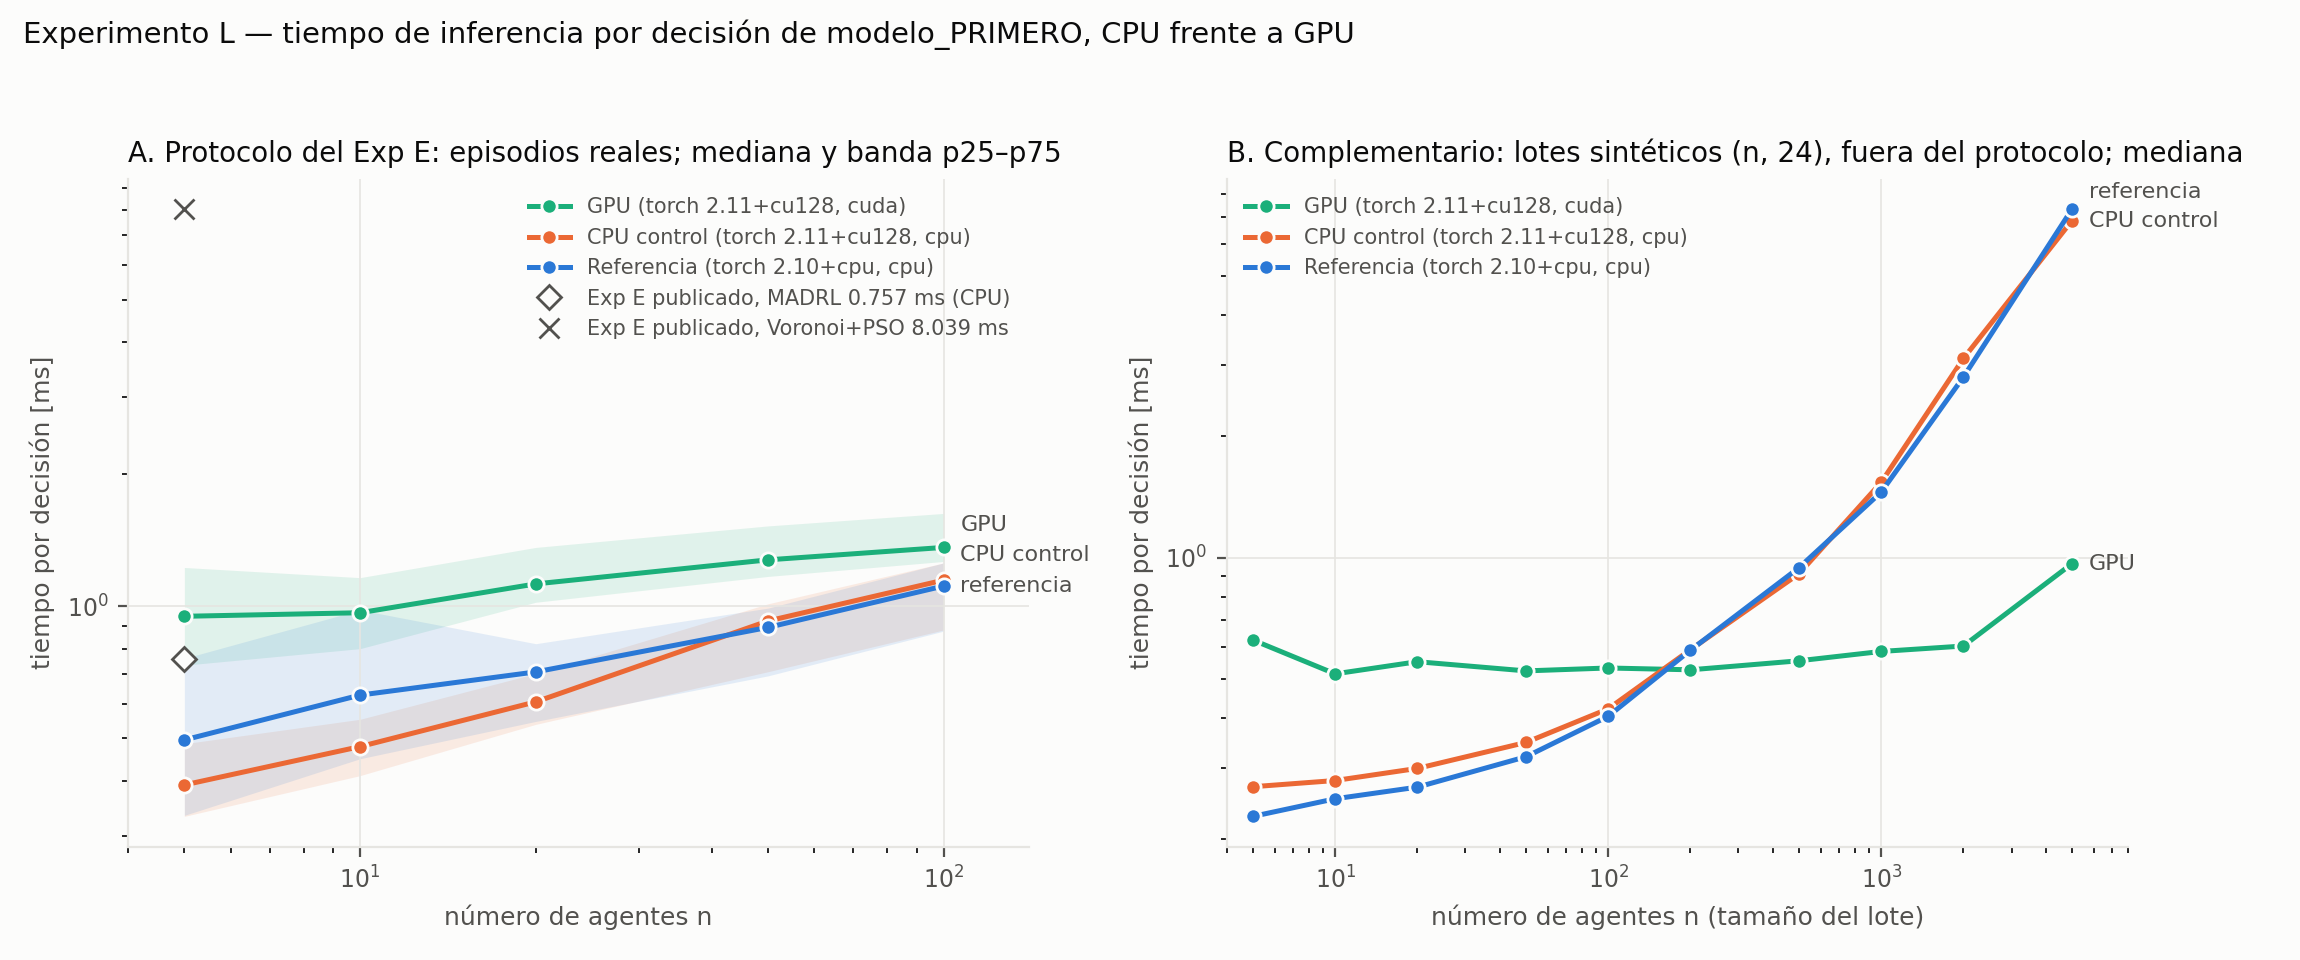
\includegraphics[width=0.98\textwidth]{fig_cpu_gpu_inferencia.png}
    \note{El panel izquierdo corresponde al protocolo de evaluación sobre
          episodios reales; el derecho, a lotes sintéticos que extienden el
          rango más allá del contemplado en este trabajo. Ambos ejes de tiempo
          emplean escala logarítmica. Elaboración propia.}
    \label{fig:cpu_gpu}
\end{figure}

Como muestra la Figura~\ref{fig:cpu_gpu}, la unidad central fue más rápida en todo el rango evaluado bajo el protocolo, y la ventaja fue máxima en la configuración de cinco agentes usada en este trabajo, con un factor de $2{.}42$. La razón baja de forma monótona con el número de agentes, como se espera, porque el costo fijo de transferencia y lanzamiento se reparte entre lotes mayores. Un barrido complementario sobre lotes sintéticos, fuera del protocolo, ubica el punto de cruce en 200 agentes.

Por lo tanto, la aceleración con hardware gráfico no aporta en ningún régimen de este trabajo, porque la configuración desplegada usa cinco agentes y la evaluación de generalización de la Sección~\ref{sec:escalabilidad} llega a 10. El sistema opera en tiempo
real sobre una unidad central convencional, empleando el $0{.}4$~\% del
presupuesto temporal disponible entre decisiones consecutivas, lo cual sustenta
la viabilidad del despliegue sobre el equipamiento disponible en el laboratorio
sin requerir hardware especializado.

\subsection*{Verificación de equivalencia}

Las políticas entrenadas sobre unidad central en ambas versiones de la
biblioteca resultaron idénticas a la configuración de referencia con seis
decimales de coincidencia. La entrenada sobre hardware gráfico difiere en
$0{.}0057$ puntos de cobertura, magnitud comprendida dentro de la variabilidad
entre semillas documentada en la Sección~\ref{sec:variabilidad_semillas}. Dicha
diferencia es esperable y no constituye un error: la aritmética de punto
flotante no es idéntica entre dispositivos, de modo que la reproducibilidad bit
a bit no se preserva al cambiar de hardware.

Debe consignarse que las mediciones se realizaron sobre un equipo que ejecutaba
simultáneamente otras aplicaciones. La ocupación del procesador se muestreó
durante cada corrida y se reporta junto a cada cifra en los artefactos del
experimento; las conclusiones se sostienen sobre las medianas por iteración,
menos sensibles a dicha contención que los totales de corrida.

Las comparaciones anteriores están sujetas a cuatro asimetrías que se declaran
de manera explícita. La arquitectura de Voronoi y PSO accede a las posiciones
globales de todos los agentes, mientras la política MADRL opera únicamente con
observación local dentro de su radio de comunicación, lo cual favorece a la
línea base y torna conservadora la comparación. En sentido inverso, los
parámetros de la arquitectura heurística se fijaron por diseño siguiendo el
trabajo previo, sin sintonización automática, frente a las 20 pruebas de
optimización bayesiana de la política neuronal; el espacio de acción de esta
última admite velocidad lineal negativa, mientras la ley de seguimiento de la
arquitectura heurística la restringe a valores no negativos; y las dos
estrategias heurísticas emplean ganancias distintas en su ley de seguimiento,
por lo que entre ambas difiere tanto la decisión de destino como el control de
bajo nivel.

% -----------------------------------------------------------------------------
\section{Robustez frente a la degradación de la información de pose}
\label{anx:robustez}
% -----------------------------------------------------------------------------

Esta sección desarrolla el barrido descrito en la
Sección~\ref{sec:robustez_pose}.

% =============================================================================

Las secciones anteriores evaluaron el sistema con información de pose exacta. En la plataforma física esa información viene de un sistema de captura de movimiento cuya cadena de captura, red y procesamiento agrega incertidumbre de medición y latencia variable. Para conocer la tolerancia del sistema a esa degradación antes de usar tiempo de laboratorio, se hizo un barrido sobre ambos factores.

\subsection*{Diseño}

La degradación se aplica a la pose en el momento en que se recibe, antes de que ningún componente la use. Por eso, tres componentes reciben la pose degradada, que son el entorno, el filtro de barrera y el detector del comportamiento de recuperación. Esta decisión es la que hace válido el experimento, porque reproduce la condición del despliegue, en el que ningún componente conoce la pose verdadera. Todas las métricas físicas, como las colisiones, las distancias a las paredes y la detección de atascamiento, se calculan en cambio sobre las poses reales.

El ruido posicional se modela como una perturbación gaussiana cuya desviación
$\sigma_{\text{pos}}$ toma los valores de 0, 5, 10 y 20~mm. El error angular no
se sortea por separado, sino que se deriva del posicional, porque un cuerpo
rígido cuyos marcadores están separados una distancia $L$ convierte un error de
posición por marcador en un error de orientación de aproximadamente
$\sigma_{\text{pos}}/L$. Con $L = 0{.}15$~m, los 20~mm corresponden a
$10{.}8^\circ$. Este acoplamiento reproduce el sistema real, en el que ambos
errores tienen el mismo origen, y su magnitud angular es unas tres veces la
usada en la aleatorización de dominio del entrenamiento.

La latencia se implementa como cola: el coordinador emplea la pose recibida
$N$ decisiones antes, con $N \in \{0,\, 1,\, 3\}$, adicional al retardo
estructural de una decisión que la propia arquitectura introduce. Tres
decisiones corresponden a $300$~ms.

El diseño es factorial completo, de 12 configuraciones sobre 18 semillas, evaluadas sobre la configuración final con cinco agentes en el
simulador con dinámica de contacto.

\subsection*{Resultados}

El Cuadro~\ref{tab:robustez} recoge el desempeño en los vértices del barrido.

\begin{table}[h]
    \centering\captionsetup{width=0.9\linewidth}
    \caption{Desempeño de la configuración final bajo degradación de la
             información de pose}
    \begin{tabular}{lcccc}
        \textbf{Magnitud} & \textbf{Sin} & $\sigma = 20$~mm &
        $N = 3$ & \textbf{Ambos} \\
        & \textbf{degradar} & & & \\
        \hline
        Agente-episodios con atascamiento & $0/90$ & $0/90$ & $0/90$
            & $0/90$ \\
        Agente-episodios con contacto & $0/90$ & $0/90$ & $0/90$ & $0/90$ \\
        Colisiones entre agentes & $0$ & $0$ & $0$ & $0$ \\
        Distancia mínima a pared [m] & $0{.}149$ & $0{.}098$ & $0{.}084$
            & $0{.}092$ \\
    \end{tabular}
    \note{Sobre la totalidad del barrido —12 configuraciones, 1\,080
          agente-episodios— no se registró atascamiento alguno ni contacto con
          las paredes. La distancia mínima corresponde al peor caso de cada
          configuración, medida sobre las poses reales. Elaboración propia.}
    \label{tab:robustez}
\end{table}

El sistema no falla en ningún punto del rango evaluado. Sobre las 12 configuraciones, equivalentes a 1\,080 agente-episodios, no se registró
atascamiento, contacto con paredes ni colisión entre agentes. La distancia
mínima al límite del área desciende de $0{.}149$ a $0{.}084$~m en el peor caso,
lo cual mantiene el chasis —de $0{.}075$~m de radio— sin contacto, aunque con
un margen que se reduce a $9$~mm.

\subsection*{Tres mecanismos que resuelven el mismo equilibrio}

El resultado anterior admite una lectura que no resulta evidente. El
comportamiento de recuperación consume la misma pose degradada que el resto del
sistema, y su detección de estancamiento depende del desplazamiento medido. Con
ruido apreciable dicho desplazamiento nunca se anula, de modo que la condición
de detección deja de satisfacerse y la maniobra no se activa. El
Cuadro~\ref{tab:mecanismos} recoge el efecto.

\begin{table}[h]
    \centering\captionsetup{width=0.85\linewidth}
    \caption{Activaciones del comportamiento de recuperación según la
             degradación aplicada}
    \begin{tabular}{lcc}
        \textbf{Condición} & \textbf{Naturaleza} &
        \textbf{Activaciones por episodio} \\
        \hline
        Sin degradar & deliberada & $9{.}1$ \\
        Ruido de pose ($\sigma \geq 5$~mm) & incidental & $0$ \\
        Latencia de tres decisiones & incidental & $0{.}6$ \\
    \end{tabular}
    \note{Elaboración propia.}
    \label{tab:mecanismos}
\end{table}

Que el sistema no falle pese a la desactivación de la capa de recuperación
obedece a que tanto el ruido como la latencia rompen, de manera incidental, el
mismo equilibrio que dicha capa fue diseñada para resolver. Una pose ruidosa
desplaza el punto de operación del problema de optimización entre decisiones
consecutivas, y una pose retrasada conduce a que el filtro responda a una
configuración que ya no es la actual; en ambos casos el sistema abandona el
punto de equilibrio sin intervención deliberada.

De ello no se sigue que la capa de recuperación resulte prescindible. Es el
único de los tres mecanismos cuyo comportamiento se encuentra caracterizado:
opera sobre el $2$\,\% de las decisiones, ninguna de sus activaciones agota el
tope de duración, y el filtro modifica su acción con magnitud media de
$0{.}037$. Prescindir de ella supondría delegar el restablecimiento del
progreso en una propiedad no especificada del sistema de captura, que podría
modificarse con una recalibración o un cambio de montaje de los marcadores.

\subsection*{Alcance del resultado}

El resultado tiene tres limitaciones.

La primera tiene que ver con el eje evaluado. La degradación aplicada corresponde a la cadena de percepción, es decir, al intervalo entre la captura de una pose y su disponibilidad para el coordinador. La cadena de actuación, que es el intervalo entre el envío de un comando y el inicio del movimiento, es un trayecto distinto que este experimento no evalúa y que se aborda en la Sección~\ref{sec:agenda_robotat}.

La segunda concierne al acoplamiento angular. Los umbrales deben enunciarse
como desviación posicional con una constelación de marcadores de
$L = 0{.}15$~m, dado que una constelación distinta transformaría el mismo
error posicional en un error angular diferente.

La tercera concierne a la generalidad respecto del cardinal. La evaluación se
realizó con cinco agentes, y la Sección~\ref{sec:escalabilidad} establece que
la dependencia del sistema respecto de las condiciones de borde varía con el
número de agentes. Los umbrales aquí determinados no admiten, por tanto,
extrapolación directa a otras densidades.

% =============================================================================

% -----------------------------------------------------------------------------
\section{Generalización a distinto número de agentes}
\label{anx:escalabilidad}
% -----------------------------------------------------------------------------

Esta sección desarrolla la evaluación descrita en la
Sección~\ref{sec:escalabilidad}.

% =============================================================================

La sección anterior mostró que la tasa de atascamiento crece con la densidad de agentes, pero esa evaluación mezcla dos efectos, la generalización de la política a un número de agentes distinto del de entrenamiento y la degradación por saturación espacial en un área fija. Para aislar el primero, se evaluó la política en el entorno de entrenamiento, sin dinámica de contacto, de modo que la única variable fuera el número de agentes, con cinco tamaños de enjambre, las dos condiciones de borde y las mismas 100 semillas del protocolo.

El interés de esta evaluación reside en que el esquema de parámetros
compartidos descrito en la Sección~\ref{sec:encoder} admite, por construcción,
la ejecución con un número arbitrario de agentes: el codificador de
representación invariante promedia sobre los vecinos visibles, de modo que la
dimensión de la observación no depende del cardinal. Dicha propiedad se
enuncia en la literatura~\cite{huttenrauch2019deep}, pero no había sido
verificada sobre el sistema del presente trabajo.

\subsection*{Cobertura y cobertura por agente}

El Cuadro~\ref{tab:escalabilidad} recoge los resultados. La cobertura total
crece de manera monótona con el cardinal, lo cual resulta trivial: más agentes
observan más área. La magnitud informativa es la cobertura por agente, que
cuantifica la eficiencia individual y permite detectar si la política mantiene
su comportamiento fuera del régimen de entrenamiento.

\begin{table}[h]
    \centering\captionsetup{width=0.80\linewidth}
    \caption{Desempeño de la política en función del número de agentes
             (100 semillas por celda, entorno de entrenamiento)}
    \begin{tabular}{lccccc}
        \textbf{Agentes} & \textbf{Cobertura} & \textbf{Cobertura} &
        \textbf{Colisiones} & \textbf{Colisiones} & \textbf{Fracción con} \\
        & \textbf{AoI} & \textbf{por agente} & $0{.}15$~m & $0{.}22$~m &
        \textbf{vecino visible} \\
        \hline
        \multicolumn{6}{l}{Reflexión elástica (condición de
        entrenamiento)} \\
        $2$  & $0{.}3785$ & $0{.}1892$ & $0{.}01$ & $0{.}02$ & $0{.}103$ \\
        $3$  & $0{.}5183$ & $0{.}1728$ & $0{.}06$ & $0{.}09$ & $0{.}190$ \\
        $5$  & $0{.}6813$ & $0{.}1363$ & $0{.}21$ & $0{.}32$ & $0{.}351$ \\
        $7$  & $0{.}7582$ & $0{.}1083$ & $0{.}72$ & $1{.}15$ & $0{.}513$ \\
        $10$ & $0{.}7967$ & $0{.}0797$ & $2{.}70$ & $4{.}43$ & $0{.}740$ \\
        \multicolumn{6}{l}{} \\
        \multicolumn{6}{l}{Borde bloqueante} \\
        $2$  & $0{.}1258$ & $0{.}0629$ & $0{.}00$ & $0{.}00$ & $0{.}054$ \\
        $3$  & $0{.}2429$ & $0{.}0810$ & $0{.}04$ & $0{.}05$ & $0{.}129$ \\
        $5$  & $0{.}4516$ & $\mathbf{0{.}0903}$ & $0{.}12$ & $0{.}17$ & $0{.}263$ \\
        $7$  & $0{.}5791$ & $0{.}0827$ & $0{.}48$ & $0{.}74$ & $0{.}394$ \\
        $10$ & $0{.}6681$ & $0{.}0668$ & $1{.}74$ & $2{.}68$ & $0{.}643$ \\
    \end{tabular}
    \note{La política fue entrenada con cinco agentes. La fracción con vecino
          visible corresponde a la proporción de decisiones en que el bloque de
          vecindad de la observación es no nulo. Elaboración propia.}
    \label{tab:escalabilidad}
\end{table}

\begin{figure}[h]
    \centering\captionsetup{width=0.85\linewidth}
    \caption{Cobertura AoI total y por agente en función del número de agentes,
             bajo ambas condiciones de borde}
    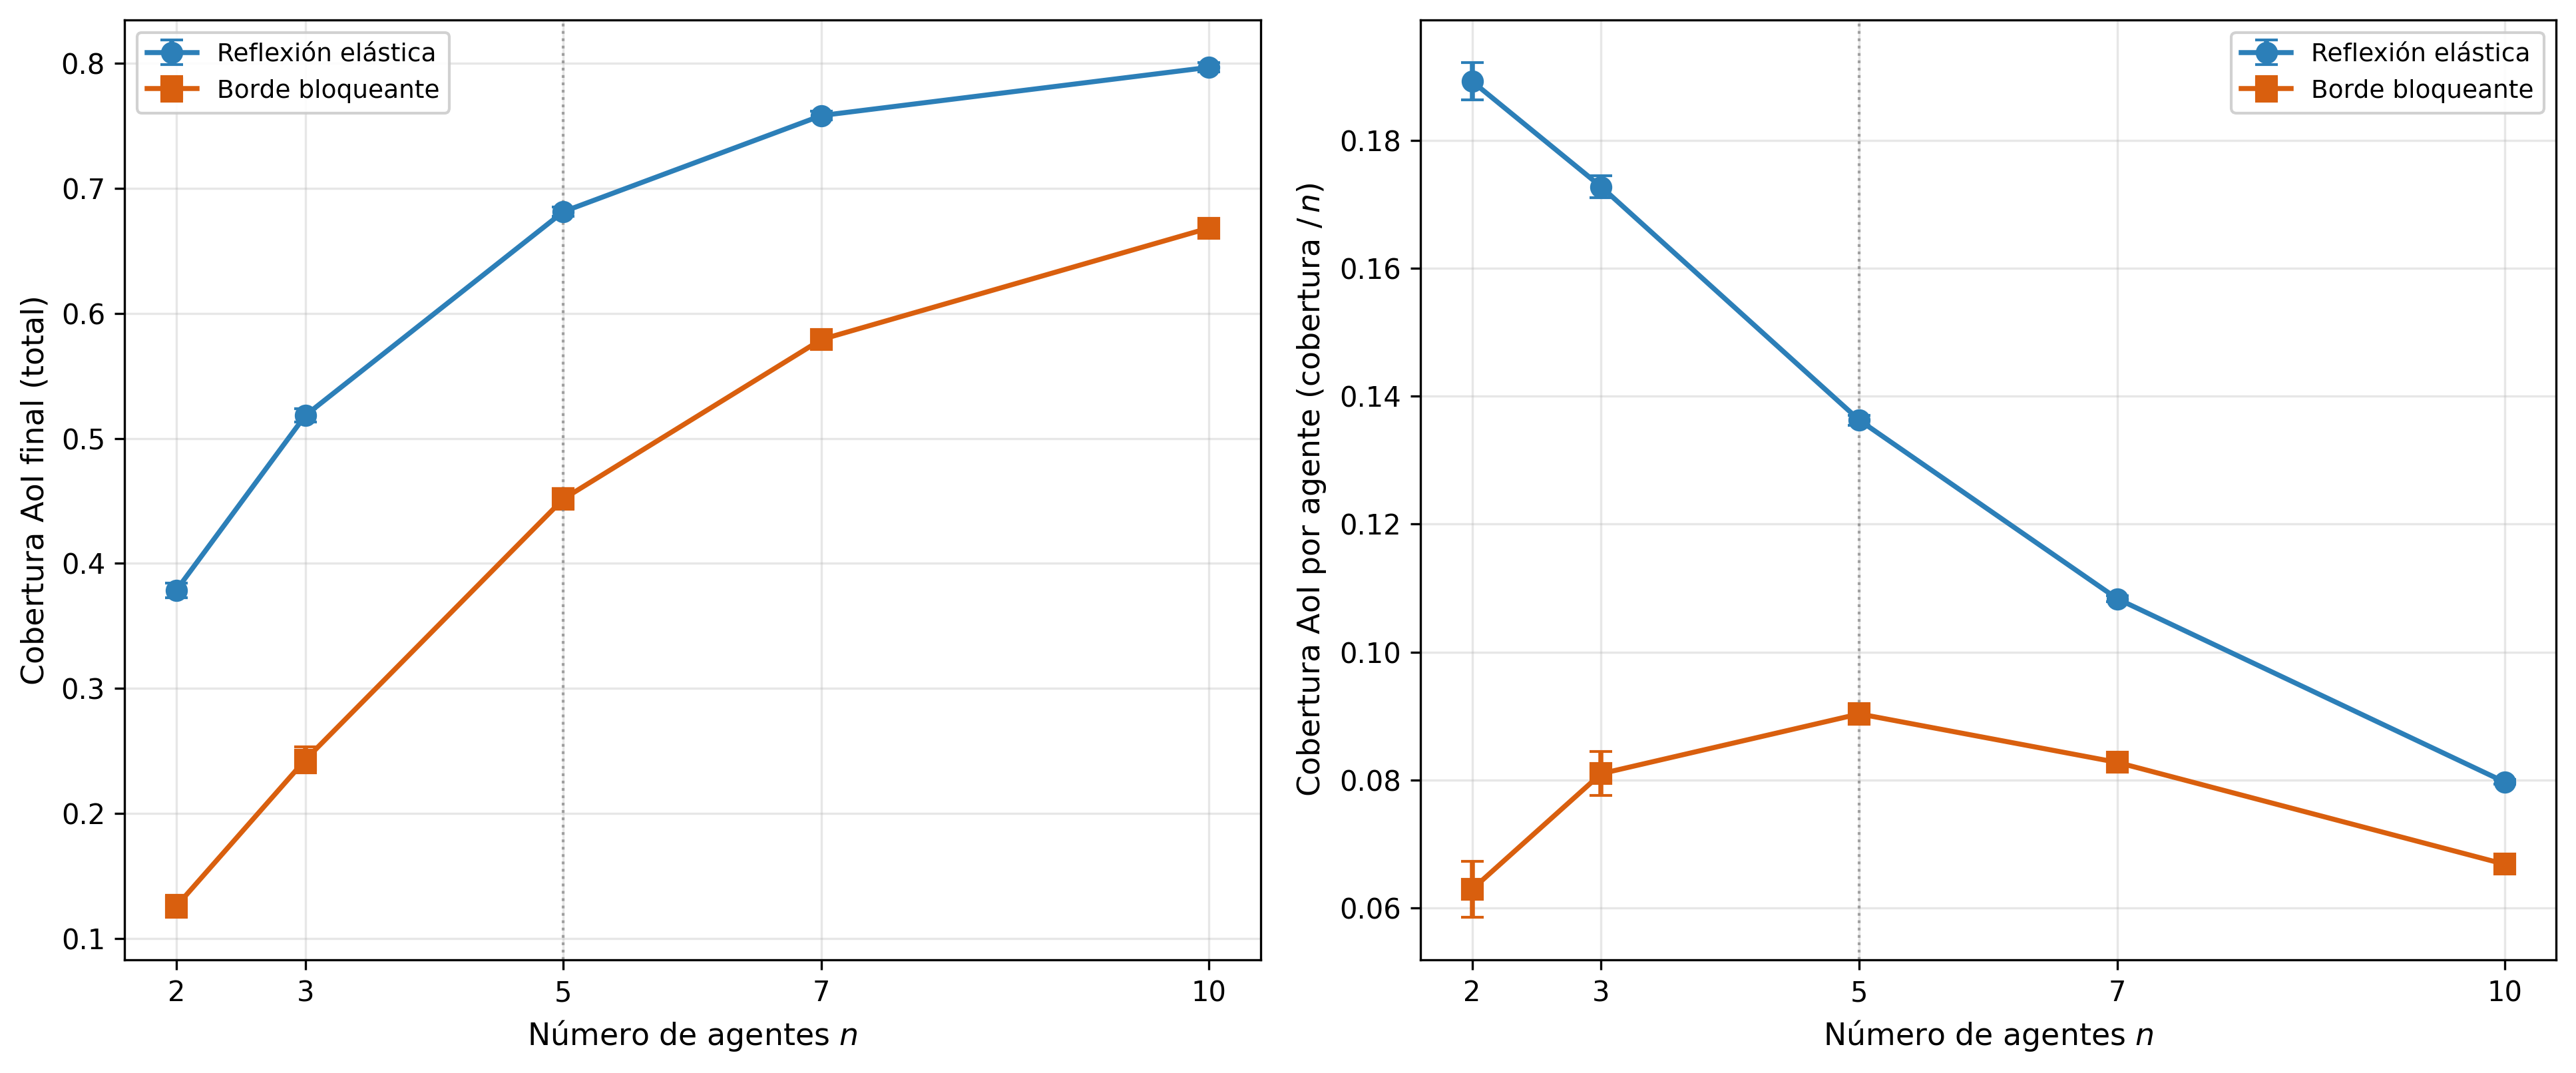
\includegraphics[width=0.80\textwidth]{fig_escalabilidad_cobertura.png}
    \note{El panel izquierdo recoge la cobertura total, cuyo crecimiento con el
          cardinal resulta esperable. El panel derecho recoge la cobertura por
          agente, que es la magnitud informativa. Las barras corresponden al
          intervalo de confianza del $95$\,\%. Elaboración propia.}
    \label{fig:escalabilidad_cobertura}
\end{figure}

Como muestra la Figura~\ref{fig:escalabilidad_cobertura}, bajo la condición de entrenamiento la cobertura por agente baja de forma monótona y suave, de $0{.}189$ con 2 agentes a $0{.}080$ con 10, sin discontinuidades. Esa caída no indica una falla, porque en un área fija el solapamiento entre las regiones observadas por agentes cercanos aumenta con la densidad, y una parte de la caída es geométrica y no se debe a la política. La ausencia de quiebres en la curva
indica que la política mantiene un comportamiento cualitativamente equivalente
en la totalidad del rango evaluado.

Bajo la condición de borde bloqueante, en cambio, la curva no es monótona y tiene un máximo en el número de agentes del entrenamiento. Las comparaciones pareadas por semilla confirman los dos lados de ese máximo. Frente a tres agentes, la diferencia fue de $0{.}0094$, con intervalo de confianza del $95$\,\% de $[0{.}0057,\, 0{.}0130]$ y 74 semillas favorables de 100, y frente a siete agentes, de $0{.}0076$, con intervalo $[0{.}0058,\, 0{.}0094]$ y 81 semillas favorables. Bajo reflexión elástica el mismo contraste es monótono, porque cinco agentes rinden menos que tres, de modo que el máximo aparece solo fuera de la condición de entrenamiento.

Este resultado admite la siguiente interpretación: la política generaliza a
cardinales distintos mientras opera dentro de su distribución de
entrenamiento, pero al modificarse la dinámica de bordes su desempeño se
optimiza en el cardinal con el que fue entrenada. Constituye, por tanto,
evidencia adicional de que la política incorporó características específicas
de su configuración de entrenamiento, en línea con la dependencia respecto de
la condición de borde establecida en la Sección~\ref{sec:gap_paredes}. Debe
señalarse que el máximo se identifica sobre los cardinales muestreados, sin que
el diseño permita determinar su ubicación exacta.

\subsection*{Activación del mecanismo de vecindad}

La última columna del Cuadro~\ref{tab:escalabilidad} recoge la proporción de
decisiones en que el agente dispone de al menos un vecino dentro de su radio de
comunicación. Dicha magnitud es exacta y no aproximada: el bloque de vecindad
es nulo si y solo si no existen vecinos visibles, dado que la componente de
distancia del descriptor es estrictamente positiva para todo vecino.

\begin{figure}[h]
    \centering\captionsetup{width=0.75\linewidth}
    \caption{Proporción de decisiones con al menos un vecino visible, en
             función del número de agentes}
    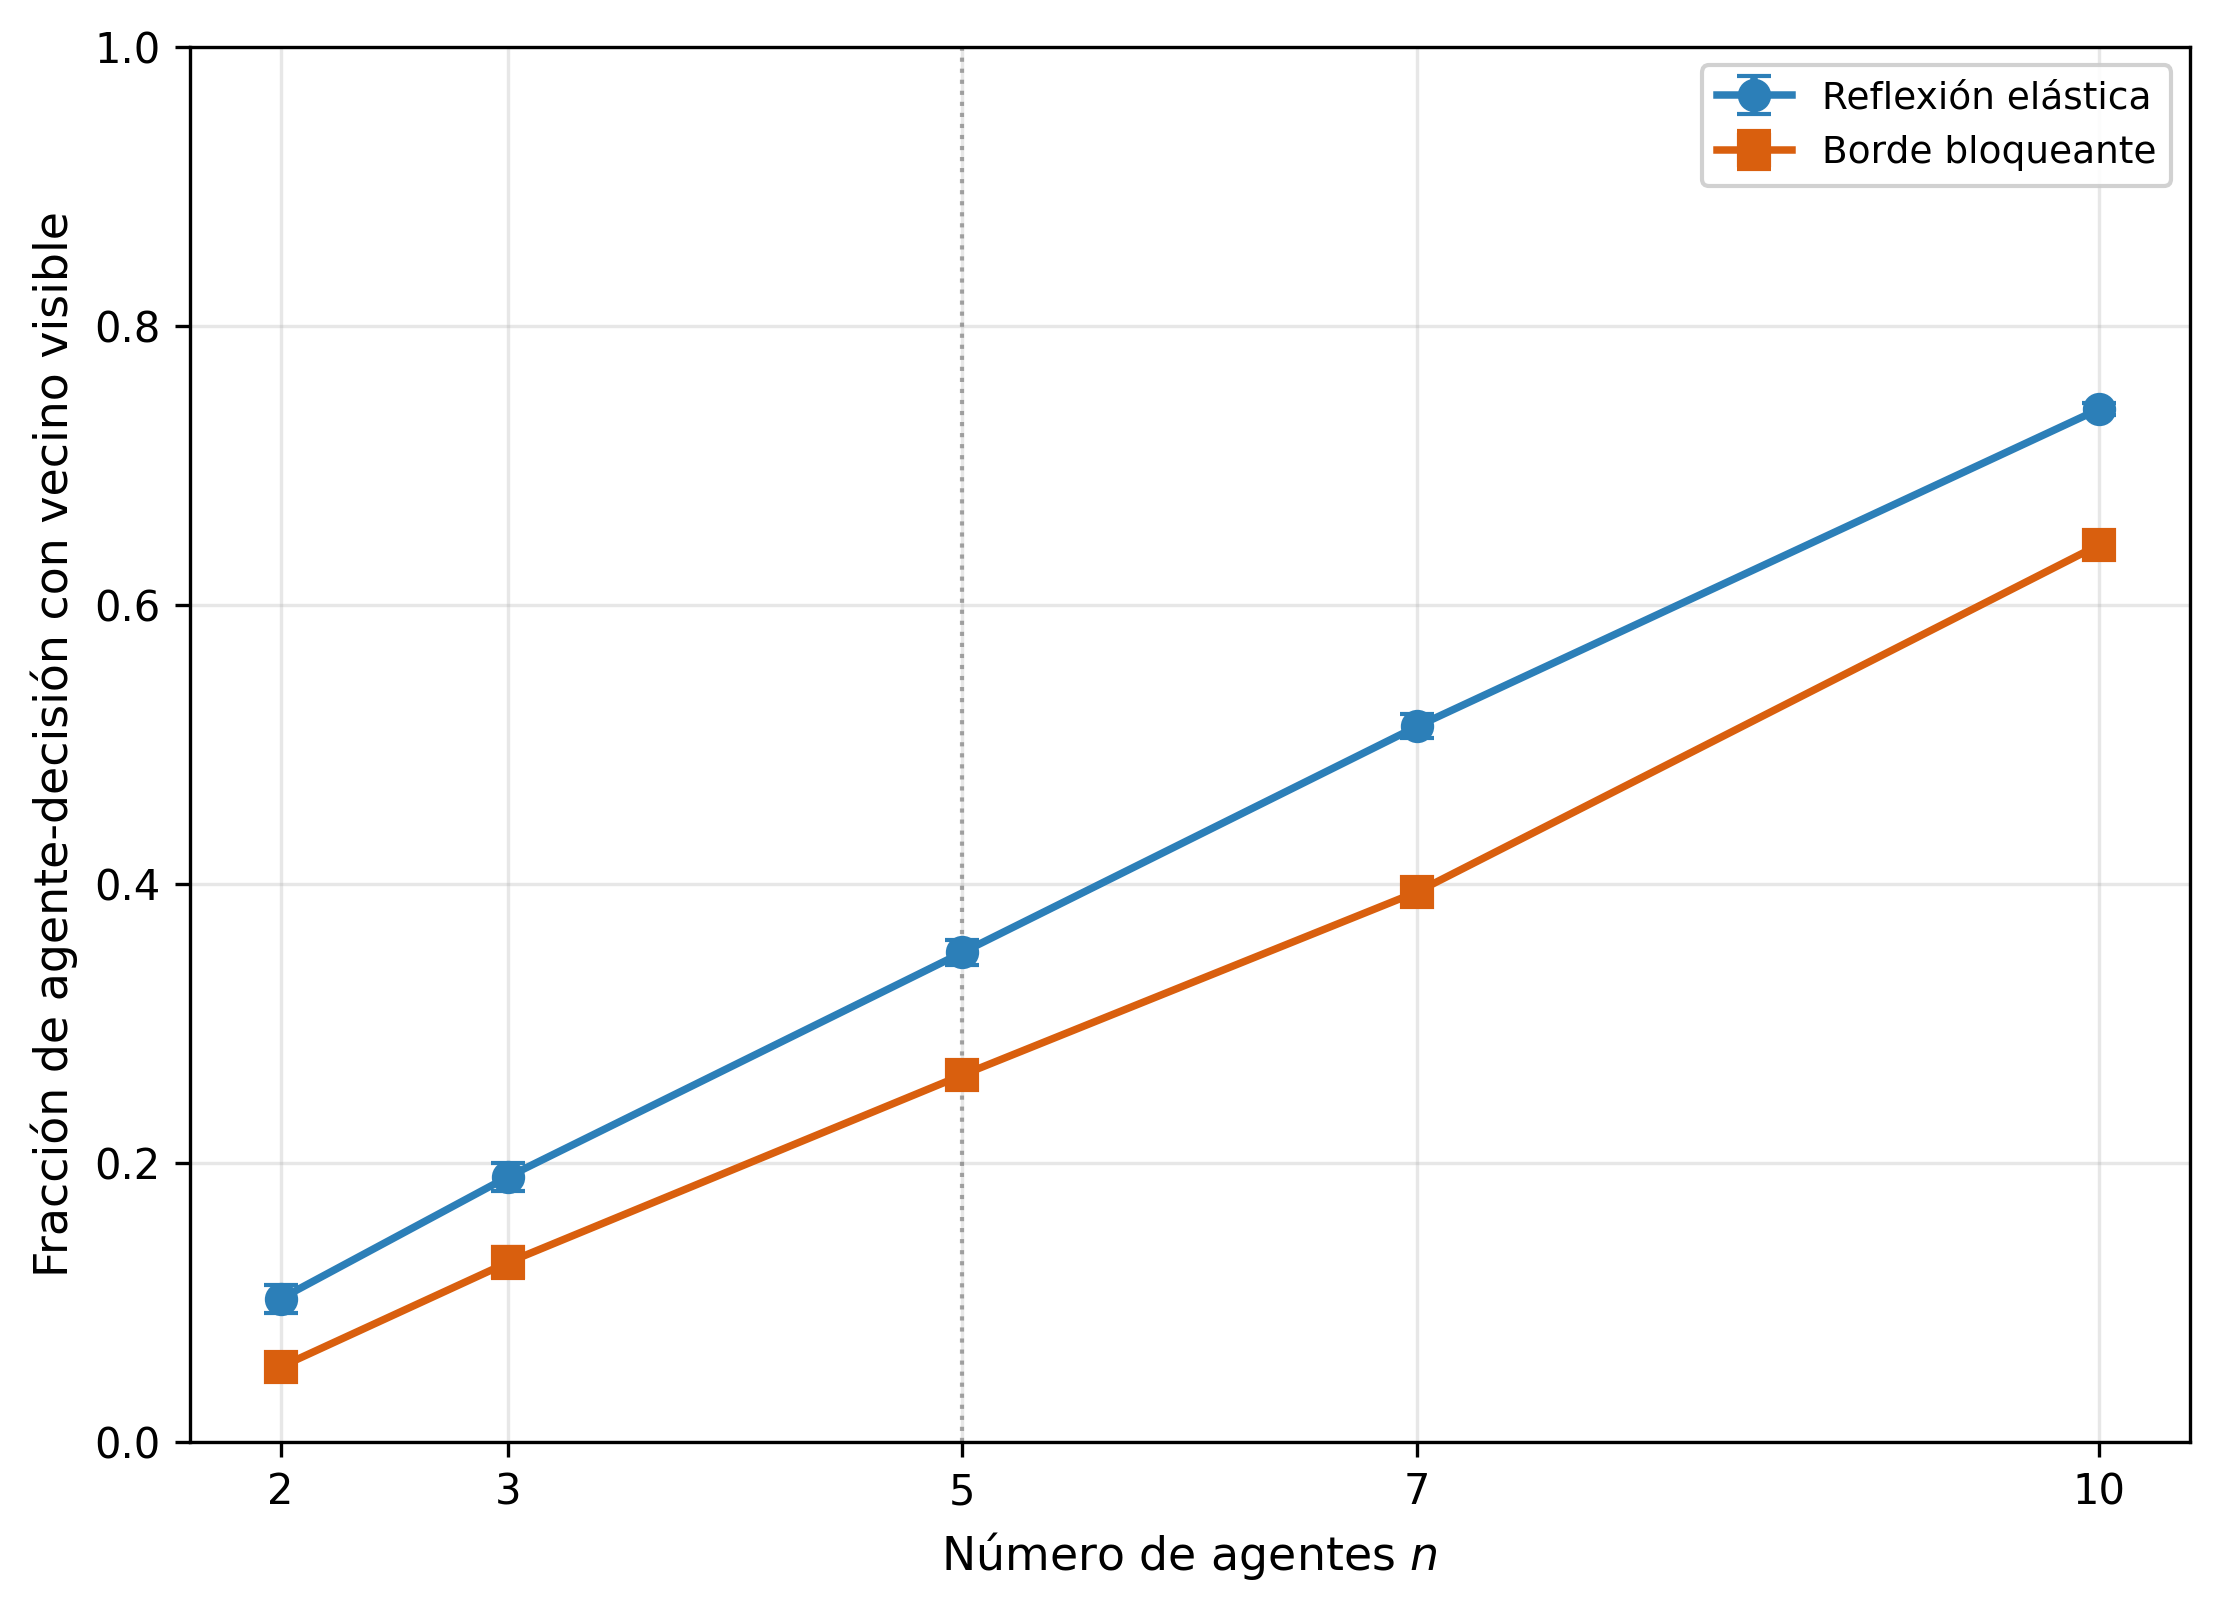
\includegraphics[width=0.80\textwidth]{fig_escalabilidad_embedding.png}
    \note{Elaboración propia.}
    \label{fig:escalabilidad_embedding}
\end{figure}

La Figura~\ref{fig:escalabilidad_embedding} muestra que el crecimiento es aproximadamente lineal, de $0{.}103$ con 2 agentes a $0{.}740$ con 10 bajo reflexión elástica. En el régimen de entrenamiento, el mecanismo de coordinación actúa solo en el $35$\,\% de las decisiones, y en las dos terceras partes restantes el agente decide sin información sobre sus pares. La coordinación observada sale, por lo tanto, de una fracción minoritaria de las decisiones, lo que es coherente con el radio de comunicación de $1{.}0$~m sobre un área de
$3 \times 3$~m.

\subsection*{Escalamiento de la tasa de colisiones}

\begin{figure}[h]
    \centering\captionsetup{width=0.85\linewidth}
    \caption{Tasa de colisiones en función del número de agentes, bajo ambos
             umbrales y ambas condiciones de borde}
    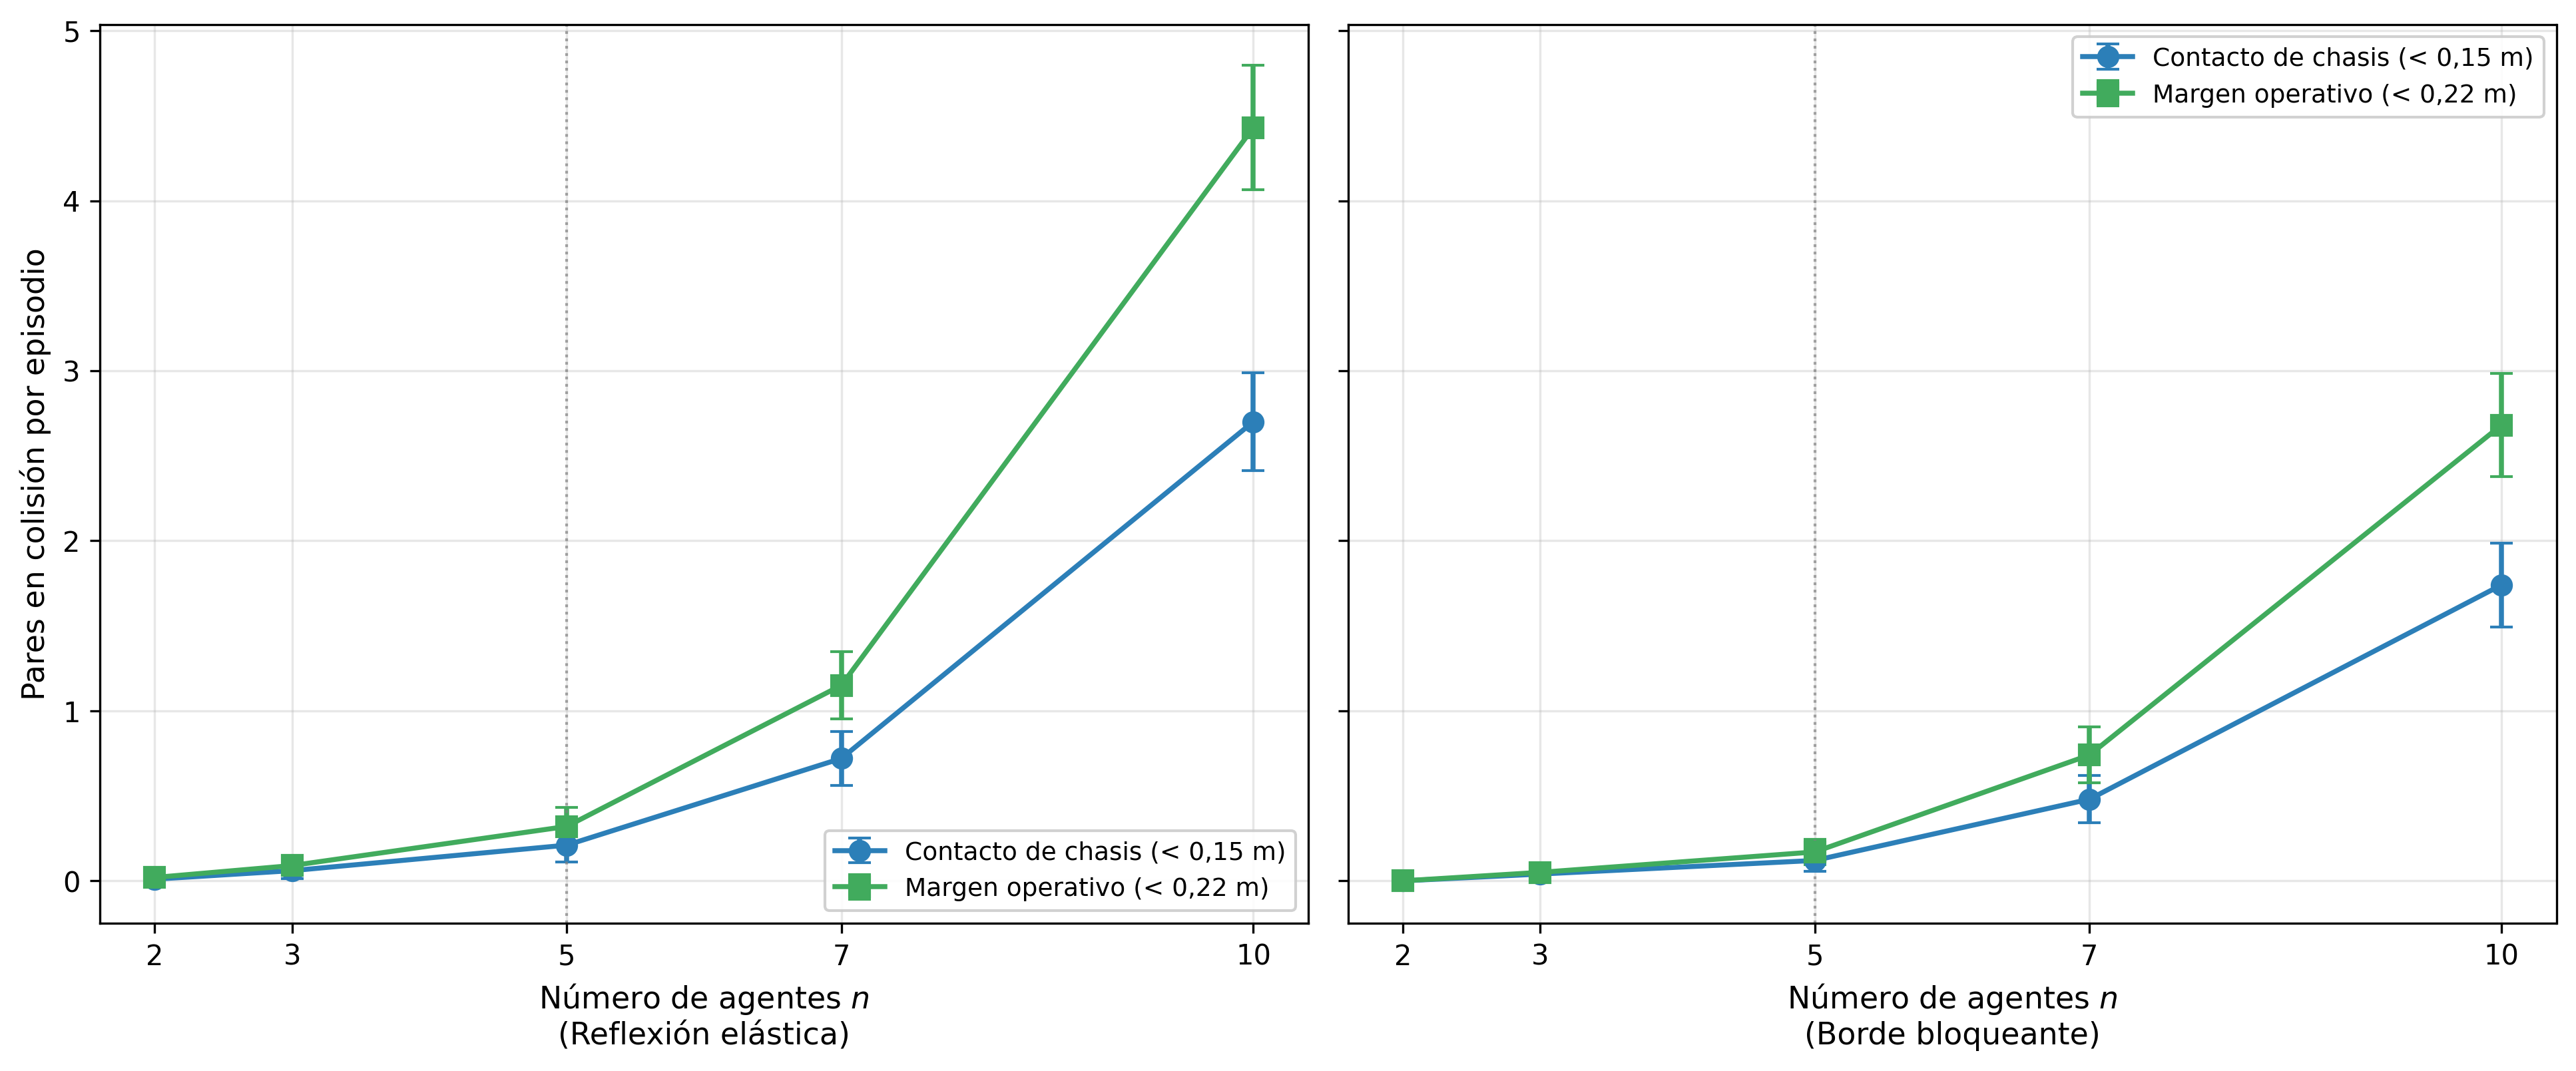
\includegraphics[width=0.80\textwidth]{fig_escalabilidad_seguridad.png}
    \note{Elaboración propia.}
    \label{fig:escalabilidad_seguridad}
\end{figure}

La generalización observada en cobertura no se extiende a la seguridad. Como muestra la Figura~\ref{fig:escalabilidad_seguridad}, entre 5 y 10 agentes la tasa de colisiones subió de $0{.}21$ a $2{.}70$ pares por episodio, un factor de $12{.}9$ al duplicar el número de agentes. Ese crecimiento es mayor que el del número de pares posibles, que solo pasa de 10 a 45, un factor de $4{.}5$.

El mecanismo está en la penalización de la ecuación~\eqref{eq:penalizacion_cbf}, que actúa sobre la distancia al vecino más cercano, de modo que su magnitud no aumenta cuando un
agente se encuentra simultáneamente próximo a varios pares. Al incrementarse la
densidad, la señal de aprendizaje que desalienta la proximidad no escala con el
número de encuentros simultáneos, y el comportamiento de evitación resulta
insuficiente. La consecuencia práctica es que el despliegue con cardinales
superiores al de entrenamiento requeriría, o bien la capa de filtrado descrita
en la Sección~\ref{sec:filtro_cbf}, o bien un reentrenamiento con una
penalización sensible al número de vecinos próximos.

\subsection*{Dependencia de la condición de borde en función del cardinal}

Un resultado adicional condiciona el alcance de los experimentos de robustez
presentados en las secciones anteriores. La degradación producida por la
sustitución de la condición de borde no es constante respecto del cardinal:
asciende al $66{.}8$\,\% con 2 agentes, al $33{.}7$\,\% con 5 y al $16{.}1$\,\% con 10, con intervalos de confianza que excluyen el cero en la
totalidad de los casos. La dependencia respecto de la dinámica de bordes es,
por tanto, más acusada cuanto menor es el número de agentes, lo cual resulta
coherente con que un enjambre reducido alcanza los límites del área con mayor
frecuencia relativa por carecer de la restricción impuesta por sus pares.

En consecuencia, los resultados de degradación reportados en la
Sección~\ref{sec:gap_paredes}, obtenidos con cinco agentes, no admiten
extrapolación directa a otros cardinales.

% =============================================================================

% -----------------------------------------------------------------------------
\section{Variantes de reentrenamiento bajo condiciones de borde}
\label{anx:reentrenamiento}
% -----------------------------------------------------------------------------

Esta sección desarrolla las tres variantes resumidas en la
Sección~\ref{sec:reentrenamiento}.

% =============================================================================

Establecido que la discrepancia de bordes constituye la causa del
atascamiento, se evaluaron tres modificaciones sucesivas de la dinámica de
borde durante el entrenamiento, cada una dirigida a un aspecto distinto de la
discrepancia. Todas emplearon la configuración de hiperparámetros de
referencia y un presupuesto de 200\,000 pasos, y se evaluaron sobre el mismo
protocolo.

\subsection*{Sustitución de la reflexión por bloqueo}

La primera variante sustituye la reflexión elástica por un recorte de la
posición a los límites del área de trabajo, sin inversión del rumbo. La
política resultante reduce la fracción de tiempo contra el borde de $0{.}5117$
a $0{.}0541$, esto es, un factor de $9{.}5$, y alcanza una cobertura
estadísticamente equivalente a la de la configuración de referencia evaluada
bajo la misma condición: la diferencia pareada sobre las 100 semillas es de
$-0{.}0171$ con un intervalo de confianza del $95$\,\% de
$[-0{.}0351,\, 0{.}0010]$, que incluye el cero.

En el simulador con dinámica de contacto y un robot, esta política reduce el
atascamiento de $18/18$ a $3/18$ episodios, incrementa el tiempo hasta el
primer atascamiento de $11{.}8$ a $31{.}3$~s, y eleva la distancia media al
borde de $0{.}0745$ a $0{.}5125$~m. La evitación aprendida transfiere, por
tanto, a la dinámica de contacto.

\subsection*{Alineación geométrica del límite}

La segunda variante incorpora el radio del chasis, recortando la posición del
centro al intervalo $[r,\, W-r]$ con $r = 0{.}075$~m, de modo que el límite
del entorno coincida con el punto en que el cuerpo físico entra en contacto
con la pared. Se evaluó adicionalmente una penalización graduada por
proximidad, con pesos $\lambda_{\text{par}} \in \{0,\, 1,\, 3\}$, según recoge
el Cuadro~\ref{tab:barrido_lambda_pared}.

\begin{table}[h]
    \centering\captionsetup{width=0.85\linewidth}
    \caption{Efecto de la penalización por proximidad a las paredes
             (evaluación en el entorno de entrenamiento)}
    \begin{tabular}{lccc}
        $\lambda_{\text{par}}$ & \textbf{Cobertura AoI} &
        \textbf{Cobertura del anillo} & \textbf{Colisiones/ep.} \\
        \hline
        $0$ & $\mathbf{0{.}5114 \pm 0{.}0757}$ & $0{.}4565$
            & $\mathbf{0{.}17}$ \\
        $1$ & $0{.}3822 \pm 0{.}0960$ & $0{.}2701$ & $3{.}72$ \\
        $3$ & $0{.}1659 \pm 0{.}0432$ & $0{.}1693$ & $9{.}44$ \\
    \end{tabular}
    \note{La cobertura del anillo corresponde a la banda perimetral de
          $0{.}30$~m adyacente a las paredes. Elaboración propia.}
    \label{tab:barrido_lambda_pared}
\end{table}

La penalización fue contraproducente. Al desalentar la cercanía a las paredes, el enjambre se concentra hacia el centro del área de trabajo, lo que tiene dos consecuencias a la vez. La cobertura de la banda perimetral empeora, y la tasa de colisiones entre agentes sube en un factor mayor que 50. Es el mismo patrón no monótono descrito en el Capítulo~\ref{cap:resultados} para el peso de penalización por proximidad entre agentes, ahora en otro término de la función de recompensa, en el que aumentar un término de penalización empeora la misma métrica que ese término busca proteger.

Sin penalización, la alineación geométrica produce la mayor cobertura obtenida
en el entorno de entrenamiento ($0{.}5114$). Sin embargo, su evaluación en el
simulador con dinámica de contacto y cinco agentes arroja el resultado
opuesto: la tasa de atascamiento asciende a $85/90$ agente-episodios
($94{.}4$\,\%), superior a la de la variante anterior.

El registro del estado en el instante del atascamiento identifica el
mecanismo: la acción comandada previa fue la velocidad lineal máxima
en retroceso en los 85 casos, sin excepción. Al desplazar el límite a
$[r,\, W-r]$ sin penalización asociada, el contacto con la pared dejó de tener
costo alguno durante el entrenamiento: el agente puede permanecer contra el
borde mientras conserva la capacidad de rotar. La variante corrigió la
posición del límite pero eliminó el único desincentivo que restaba para
aproximarse a él.

\subsection*{Contacto con bloqueo de rotación}

La tercera variante incorpora la característica del contacto físico que las
anteriores omitían. Durante los atascamientos observados en el simulador, la
variación angular es nula de manera exacta, lo cual indica que la fricción del
chasis contra la pared bloquea también la rotación. La variante replica esta
condición: cuando el agente se encuentra en contacto y la componente normal de
su velocidad apunta hacia el exterior, la orientación no se integra durante
ese paso. La salida permanece siempre disponible, dado que reducir o invertir
la velocidad lineal restituye la rotación, de modo que no se introducen
estados absorbentes.

El entrenamiento no convergió a una política satisfactoria. La política
resultante permanece en contacto con las paredes durante el $68{.}7$\,\% de
los pasos, con una mediana de distancia al borde de exactamente $0{.}0750$~m
—el radio del chasis— y comandos de velocidad negativa en el $84{.}6$\,\% de
los pasos. En el simulador con cinco agentes, la tasa de atascamiento asciende
a $82/90$ agente-episodios ($91{.}1$\,\%).

La interpretación propuesta atribuye el fallo a la dificultad de asignar crédito que introduce la modificación. Al dejar de integrar la orientación durante el contacto, las acciones de giro no tienen efecto observable justo en los estados donde hacen falta, de modo que desaparece la señal necesaria para aprender la maniobra de recuperación allí donde se debe aplicar. La única salida disponible, que es reducir o invertir la velocidad lineal, se tiene que descubrir por exploración, sin un gradiente que la oriente.

\subsection*{Síntesis de las variantes evaluadas}

Las tres modificaciones de la dinámica de borde produjeron tasas de
atascamiento comprendidas entre el $56{.}7$\,\% y el $94{.}4$\,\% en el
simulador con dinámica de contacto y cinco agentes. Ninguna cerró la
discrepancia. La primera variante, que sustituye la reflexión por bloqueo,
resultó la más favorable de las tres, pese a ser la que menos se aproxima a la
geometría real del contacto.

Este resultado, de carácter negativo, posee valor informativo: establece que
la discrepancia de bordes no se resuelve mediante ajustes de la dinámica de
simulación dentro del presupuesto de entrenamiento empleado, y sustenta la
adopción de una capa de protección durante la ejecución como estrategia de
transferencia.

% =============================================================================

% -----------------------------------------------------------------------------
\section{Verificación del cliente sin acceso a la plataforma}
\label{anx:verificacion}

\subsection*{Verificación de la sincronía del esquema multi-agente}

\subsection*{Verificación de sincronía}

Dado que la política decide a partir de poses recibidas por un canal de
comunicación, la validez del lazo depende de que dichas poses sean recientes.
Se instrumentó, para cada decisión, la antigüedad de la pose empleada por
agente, el número de decisiones tomadas con información obsoleta y la latencia
entre la emisión de la pose y la aplicación de la acción correspondiente.

La antigüedad observada fue de un paso de simulación en la totalidad de las
decisiones, con cero decisiones basadas en información obsoleta y una latencia
media de $10{.}00$~ms, en las tres configuraciones evaluadas (uno, dos y cinco
agentes). Este retardo de un paso constituye un desfase estructural: el
simulador no garantiza el orden de ejecución entre controladores dentro de un
mismo paso, de modo que un mensaje emitido en el paso $k$ puede ser leído en
$k$ o en $k+1$ según el orden de despacho. No se registró pérdida de mensajes
ni degradación al aumentar el número de agentes, lo cual establece que la
arquitectura de comunicación no introduce limitaciones sobre el desempeño
observado.

\subsection*{Procedimiento de arranque}

El arranque presenta un riesgo simétrico: una configuración incorrecta del
mapeo de identificadores o de la transformación de marco produciría el
desplazamiento inmediato de los robots en direcciones arbitrarias. Se
incorporaron dos mitigaciones.

La primera es una verificación geométrica previa a toda actuación, que
comprueba que las cinco poses iniciales estén presentes, se encuentren dentro
del área de trabajo, guarden entre sí una separación superior al umbral de
contacto, y no se sitúen a menos de $0{.}20$~m de una pared. Esta última
condición se deriva de los resultados de la Sección~\ref{sec:gap_paredes}: la
política carece de comportamiento de recuperación aprendido y el mecanismo de
recuperación implementado requiere la intervención previa del filtro, de modo
que un agente que inicie en contacto con una pared no dispone de salida.

La segunda es una rampa de velocidad que limita los comandos al $25$\,\% de la cota durante los primeros $5$~s de operación. El
escalado preserva las garantías del filtro de barrera, dado que la condición
de invarianza se mantiene bajo multiplicación por un factor en el intervalo
unitario. Durante la rampa, las componentes de
velocidad del vector de observación no reflejan la acción efectivamente
aplicada, ya que la política recibe como observación la velocidad que comandó y no la
que se ejecutó. Durante la rampa dicha discrepancia se limita a los primeros
segundos de operación; bajo el régimen de velocidad reducido descrito en la
Sección~\ref{subsec:regimen_velocidad}, en cambio, persiste durante la
totalidad del episodio. Constituye una limitación declarada de la configuración
de despliegue y un candidato a explicar diferencias de desempeño respecto de la
simulación.

Cabe observar que el nivel de velocidad de la rampa, $0{.}078$~m/s, resulta
prácticamente coincidente con el régimen de operación del material de
referencia del laboratorio, lo cual sugiere que dicho valor constituye un
punto de partida razonable.

% -----------------------------------------------------------------------------

Esta sección desarrolla la batería de verificación descrita en la
Sección~\ref{sec:verificacion_local}.

Con el propósito de ejercitar el cliente antes de disponer de acceso al
laboratorio, se implementó un servidor local que reproduce ambos servicios de
la plataforma y admite la inyección deliberada de fallos: pérdida de
marcadores, latencia variable, interrupción de conexión y respuestas
malformadas.

Contra dicho servidor se verificó la codificación de ambos protocolos, la
conversión de unidades y su saturación, la obtención del rumbo a partir del
cuaternión, el comportamiento ante cada modo de fallo, el procedimiento de
arranque con cada condición inválida, y la ejecución del coordinador completo, política, filtro y comportamiento de recuperación, sin intervención del
simulador de Webots.

Debe precisarse el alcance de esta verificación. El servidor local reproduce
el protocolo, no la dinámica: emplea la misma cinemática ideal del entorno de
entrenamiento, de modo que ninguna de las pruebas realizadas aporta
información sobre la brecha de transferencia. Lo verificado es exclusivamente
la corrección de la capa de comunicación.

% -----------------------------------------------------------------------------
\section{Efecto del peso de penalización por proximidad}
\label{anx:lambda_cbf}
% -----------------------------------------------------------------------------

Esta sección desarrolla el barrido sobre el peso de penalización por
proximidad, cuyo resultado se enuncia en el Capítulo~\ref{cap:resultados}.

% =============================================================================
 
La correlación negativa observada entre $\lambda_{\text{cbf}}$ y el desempeño
durante la sintonización motivó un análisis específico. Se entrenó una configuración adicional, idéntica a la de referencia salvo por
el valor de dicho peso, elevado de $2{.}9655$ a $5{.}0$, y se evaluó bajo el
protocolo estándar. El Cuadro~\ref{tab:efecto_lambda_cbf} presenta la
comparación.
 
\begin{table}[h]
    \centering\captionsetup{width=0.85\linewidth}
    \caption{Efecto del peso de penalización por proximidad sobre el
             desempeño}
    \begin{tabular}{lccc}
        \textbf{Configuración} & $\lambda_{\text{cbf}}$ &
        \textbf{Cobertura AoI} & \textbf{Colisiones/ep.} \\
        \hline
        Referencia & $2{.}9655$ & $0{.}6805 \pm 0{.}0213$
            & $0{.}200 \pm 0{.}476$ \\
        Peso incrementado & $5{.}0$ & $0{.}5913 \pm 0{.}0337$
            & $0{.}433 \pm 0{.}559$ \\
    \end{tabular}
    \note{Configuraciones idénticas salvo por el peso de penalización,
          entrenadas durante 200\,000 pasos y evaluadas sobre los mismos 30 episodios deterministas bajo el protocolo unificado. Las
          colisiones corresponden a pares únicos a distancia inferior a
          $0{.}15$~m. La cifra de referencia difiere de la reportada en el Capítulo~\ref{cap:resultados} por corresponder a 30 episodios en lugar de 100, de modo que ambas columnas resulten
          comparables. Elaboración propia.}
    \label{tab:efecto_lambda_cbf}
\end{table}
 
 
El incremento del peso de penalización degradó de manera simultánea la
cobertura, en $0{.}089$ puntos, y la tasa de colisiones, que se duplicó. Este comportamiento resulta contraintuitivo,
dado que el término penalizado es precisamente el que la métrica de seguridad
cuantifica. La interpretación propuesta es que una penalización excesiva
induce políticas de evitación conservadoras que restringen el desplazamiento de
los agentes; la consiguiente reducción de la movilidad limita la cobertura y,
al concentrar a los agentes en configuraciones espaciales menos favorables,
tampoco reduce los encuentros próximos.
 
Un fenómeno análogo se observó posteriormente al introducir una penalización
por proximidad a las paredes, según se documenta en el Capítulo~\ref{cap:transferencia}. Ambas observaciones convergen en una conclusión metodológica:
los pesos de la función de recompensa interactúan de manera no monótona, de
modo que su ajuste requiere validación empírica y no admite selección por
razonamiento sobre el término penalizado de forma aislada.

% -----------------------------------------------------------------------------
\section{Material complementario del capítulo de transferencia}
\label{anx:complemento_transferencia}
% -----------------------------------------------------------------------------

Esta sección recoge el desarrollo de los apartados que el Capítulo~\ref{cap:transferencia} resume: la validación de la cadena de herramientas en Webots, el
efecto de la densidad sobre el atascamiento, el régimen de velocidad admisible,
el protocolo detallado de la sesión física, la comparación consolidada de
configuraciones, el margen de operación y el ciclo de decisión del agente.

\subsection*{Validación en el simulador Webots}

Con el propósito de validar el comportamiento de la política entrenada y de
cuantificar el primer escalón de la brecha entre simulación y realidad
(\textit{sim-to-real gap}), se implementaron dos mundos paralelos en Webots
R2025a que replican las dimensiones y condiciones operativas del laboratorio
Robotat. Ambos mundos emplean un área de trabajo de $3{.}0 \times 3{.}0$~m con paredes
de $0{.}1$~m de espesor, coincidente con el espacio de entrenamiento, y tres
objetivos dinámicos (\textit{hotspots}) representados como esferas flotantes
de colores distintos, cuyo desplazamiento se genera con el mismo simulador de
objetivos empleado durante el entrenamiento.

\subsection*{Validación de la cadena de herramientas}

El primer mundo, denominado \texttt{lab\_robotat.wbt}, implementa una
validación cinemática en la que cinco robots Pololu 3pi+ son posicionados en
cada paso por un controlador supervisor único, el cual inyecta la
pose calculada por el entorno de entrenamiento. Bajo este esquema, Webots
opera como renderizador: la política entrenada durante $200\,000$ pasos
(cobertura AoI $= 0{.}681 \pm 0{.}020$) produce las acciones $(v, \omega)$, el
entorno integra la cinemática de uniciclo ideal y el supervisor
transcribe las poses resultantes a los nodos tridimensionales. Los
\textit{hotspots} se desplazan en tiempo real siguiendo el modelo de caminata
aleatoria suave con reflexión elástica.

La corrida de validación cinemática confirmó que la política exhibe el
comportamiento coordinado esperado: los cinco agentes se distribuyen sobre el área de trabajo, convergen hacia los objetivos activos y evitan colisiones mutuas de
manera sistemática. Este resultado valida la cadena de herramientas de
inferencia —carga del modelo PPO, construcción del vector de observación de
24 dimensiones y conversión de acciones— antes de introducir la dinámica de
ruedas.


El segundo mundo, \texttt{lab\_robotat\_fisica.wbt}, introduce dinámica física
real: el robot Pololu 3pi+ opera con masa, fricción y motores de tracción
diferencial. La pose deja de ser impuesta por el supervisor y pasa a
emerger de la acción de las ruedas sobre la superficie simulada. El
controlador lee la posición del robot mediante GPS y la orientación mediante brújula, transforma ambas lecturas al marco del entorno de
entrenamiento y las inyecta a este antes de cada consulta a la política.

El modelo cinemático inverso del diferencial, recogido en la
ecuación~\eqref{eq:diff_drive_inverso} del marco teórico, traduce el par
$(v, \omega)$ producido por la política a velocidades angulares de rueda. Los
parámetros empleados son $r = 0{.}035$~m de radio de rueda y
$\ell = 0{.}07$~m de semiancho del eje, correspondientes a la geometría del
mundo simulado. Las salidas
$\dot{\varphi}_{R,L}$ se envían directamente en rad/s a los actuadores
rotacionales, sin conversión a revoluciones por minuto, unidad que corresponde
exclusivamente al canal de comunicación con el hardware físico.

La calibración del modelo de ruedas se verificó en lazo abierto mediante tres
pruebas de giro y avance, cuyos resultados se detallan en el
Anexo~\ref{anx:verificacion}. Las tres reprodujeron el comportamiento esperado
dentro de la tolerancia del simulador.

\subsection*{Efecto de la densidad sobre la tasa de atascamiento}

La sincronía del esquema se verificó antes de evaluar su desempeño, con el
resultado de que ninguna decisión se toma sobre información obsoleta y el
retardo introducido se limita a un paso de simulación, según se detalla en el
Anexo~\ref{anx:verificacion}.


La evaluación de la política sobre configuraciones de uno, dos y cinco agentes
revela que la tasa de atascamiento escala con la densidad, según recoge el
el Anexo~\ref{anx:cuadros_sim}.

El incremento no se explica únicamente por la mayor cantidad de agentes
expuestos, dado que la tasa se expresa por agente-episodio y aun así se
triplica entre una y cinco unidades. La columna de distancia al borde provee
el mecanismo: a mayor número de agentes, menor es el espacio libre disponible
y más próximos a los límites operan los robots, con lo cual aumenta la
frecuencia con que se alcanza la condición que desencadena el atascamiento.

Se evaluó la hipótesis alternativa de que la evitación entre agentes
empujara a los robots contra las paredes. El registro del estado en el
instante del atascamiento la descarta: con cinco agentes, únicamente 15 de los
51 casos presentaban un vecino dentro del radio de comunicación, y de estos
solo siete a distancia inferior a $0{.}22$~m; con dos agentes, ninguno de los
nueve casos presentaba vecino próximo. La acción comandada previa al
atascamiento fue la velocidad lineal máxima hacia la pared en la totalidad de
los casos. El mecanismo dominante es, por tanto, la discrepancia entre el
agente puntual del entorno de entrenamiento y el cuerpo con extensión física
del simulador; la densidad incrementa la exposición, no la causa.

\subsection*{Régimen de velocidad admisible}

La discrepancia de mayor consecuencia operativa concierne a los límites de
velocidad. El material de referencia del laboratorio opera con una velocidad
lineal máxima de $0{.}07$~m/s y una velocidad angular máxima de $1{.}0$~rad/s,
con saturación adicional a $200$~rpm por rueda, y consigna explícitamente
que dichos valores responden a la latencia del enlace inalámbrico. La política
del presente trabajo emite comandos de hasta $0{.}31$~m/s y $6{.}28$~rad/s,
valores tomados de las especificaciones del motor.

El Anexo~\ref{anx:calibracion} contrasta ambos regímenes expresados en
velocidades de rueda, empleando la geometría del robot físico.

La combinación más exigente del espacio de acciones de la política excede en
un factor de $1{.}83$ el límite operativo adoptado en el material de
referencia, aunque permanece dentro de la saturación del protocolo. Debe
señalarse que la cota de velocidad lineal forma parte de la normalización del
vector de observación, de modo que su modificación invalidaría el modelo
entrenado. La resolución de esta discrepancia admite tres alternativas, operar sin restricción adicional y caracterizar la respuesta, imponer una
saturación en la capa de actuación, o reentrenar con el espacio de acciones
restringido,  cuya elección se subordina a la evidencia que arroje la primera
sesión experimental.

Esta discrepancia no fue cubierta por los
experimentos de robustez de la Sección~\ref{sec:robustez_pose}: aquellos
caracterizaron la tolerancia a información de pose degradada, esto es, latencia
en la cadena de percepción, mientras que la reducción de velocidad del material
de referencia responde a latencia en la cadena de actuación. Ambos ejes son
distintos, y la determinación del segundo se incorporó al procedimiento de
calibración descrito en el Anexo~\ref{anx:latencias}.

\subsection*{Protocolo de la sesión}

Cada episodio comprende 500 decisiones a $10$~Hz, equivalentes a $50$~s de operación, en correspondencia con el protocolo empleado
en simulación. La acción comandada se escala por un factor de $0{.}40$ respecto
de la cota del espacio de acción, régimen determinado durante la calibración
como el de operación estable.

Entre episodios los robots se reposicionan autónomamente: cada unidad se
desplaza por sus propios medios hasta la pose sorteada, bajo el mismo filtro de
barrera que gobierna los episodios y con velocidades acotadas al régimen del
laboratorio. El procedimiento sitúa a las unidades con un error mediano de
posición de $0{.}026$~m en un tiempo de entre $19$ y $34$~s.

Este reposicionamiento es una condición de validez y no solo una comodidad operativa. En la campaña exploratoria, con colocación manual, las poses iniciales quedaron sistemáticamente más juntas que las del procedimiento de entrenamiento, con una distancia media al vecino más cercano de $0{.}273$~m, frente al intervalo de $0{.}64$ a $0{.}84$~m del sorteo. Con reposicionamiento autónomo, en la evaluación del 26 de septiembre, esa distancia subió a $0{.}717$~m, en el percentil 45 de la distribución de referencia, de modo que las poses iniciales son representativas de las del entrenamiento. En la evaluación del 30 de septiembre, en cinco de los 50 episodios válidos quedaron 11 robots a entre $0{.}44$ y $1{.}49$~m de su pose asignada, y esos arranques tienen algún par de robots a menos de $0{.}31$~m, el mínimo del sorteo de entrenamiento. Sin esos cinco episodios, la distribución de los arranques es compatible con la del sorteo.

Un episodio se considera válido si completa las quinientas decisiones sin
incurrir en ninguna de las condiciones de aborto automático. El 30 de septiembre resultaron válidos 50 de 57 intentos, en cinco sesiones de 11 o 12
intentos. El Anexo~\ref{anx:limitaciones} recoge las causas de descarte.

El sistema operó sobre la plataforma física con las características recogidas
en el Cuadro~\ref{tab:ejecucion_fisica}.

\begin{table}[h]
    \centering\captionsetup{width=0.9\linewidth}
    \caption{Características de la ejecución sobre el enjambre físico
             (evaluación del 30 de septiembre, 50 episodios válidos)}
    \begin{tabular}{lc}
        \textbf{Magnitud} & \textbf{Valor} \\
        \hline
        Cobertura AoI & $0{.}3452 \pm 0{.}0428$ \\
        Colisiones entre unidades & $0$ \\
        Distancia mínima al límite del área & $0{.}1317 \pm 0{.}0169$~m \\
        Violaciones del margen por episodio & $2{.}00 \pm 0{.}83$ \\
        Fracción de decisiones con intervención del filtro & $0{.}273$ \\
        Separación mínima entre unidades & $0{.}432 \pm 0{.}127$~m \\
    \end{tabular}
    \note{La desviación corresponde a la dispersión entre episodios. La
          distancia mínima se reporta como media de los mínimos por episodio.
          El intervalo de confianza del $95$\,\% de la cobertura media,
          agrupando por semilla, es $[0{.}3253,\, 0{.}3651]$. Elaboración
          propia.}
    \label{tab:ejecucion_fisica}
\end{table}

\subsection*{Comparación consolidada}

El Cuadro~\ref{tab:tabla_final} presenta las cinco configuraciones evaluadas
en el simulador con dinámica de contacto y cinco agentes, sobre las mismas 18
semillas y bajo condiciones idénticas. Al ejecutarse todas sobre la misma
física, esta comparación constituye la única directamente válida entre
variantes, dado que las evaluaciones realizadas en el entorno de entrenamiento
emplean, cada una, su propia dinámica de borde.

La configuración que combina el entrenamiento con bordes bloqueantes y el filtro de barrera de ejecución es la mejor en seguridad y en progreso, porque es la única sin ninguna colisión en las 18 semillas y tiene la menor tasa de atascamiento. También alcanza la cobertura más alta del conjunto, aunque su ventaja sobre la variante de alineación geométrica, $0{.}3199 \pm 0{.}0830$ frente a $0{.}3107 \pm 0{.}0644$, está dentro de la dispersión de ambas y por eso no sirve como criterio de selección. Ninguna variante posterior de reentrenamiento la superó en seguridad ni en progreso, con filtro o sin él. El Anexo~\ref{subsec:escape} agrega sobre esta configuración la tercera capa, que resuelve el atascamiento residual.

La variante de alineación geométrica alcanza la segunda mejor cobertura del conjunto aunque tiene la peor tasa de atascamiento. Las dos cosas son compatibles, porque los agentes que siguen operando cubren bien el área y los atascados dejan de aportar. Por eso, la cobertura sola no basta como criterio de selección para el despliegue físico.

\subsection*{Margen de operación y configuración adoptada}

El criterio operativo descrito en la
Sección~\ref{subsec:criterio_operativo} sitúa en $0{.}5$ la fracción de
intervención por encima de la cual la tasa de atascamiento resulta elevada. La
configuración adoptada opera con una fracción de $0{.}397$, de modo que dispone
de un margen aproximado de $0{.}10$ antes de alcanzarlo. Dos evaluaciones
complementarias, desarrolladas en el Anexo~\ref{anx:restricciones},
cuantifican con qué facilidad se consume dicho margen.

La primera evaluó la conveniencia de reducir el área de trabajo a
$2{.}7 \times 2{.}7$~m, motivada por la mayor precisión del sistema de captura
en la región central de su volumen. La reducción degrada el desempeño de la
configuración completa más allá de lo que la mayor densidad de agentes
explica, con un residuo de $-0{.}0204$ e intervalo de confianza del $95$\,\% de
$[-0{.}0358,\, -0{.}0050]$, y eleva la fracción de intervención a $0{.}541$. El
mecanismo es geométrico: los márgenes del filtro son magnitudes absolutas
derivadas de dimensiones físicas y no escalan con el área, de modo que un área
menor eleva la razón entre perímetro y superficie y con ella el trabajo de las
barreras de pared. Se adoptó, en consecuencia, el área original.

La segunda evaluó la incorporación de obstáculos estáticos, tratados como
barreras adicionales del filtro. Dicha evaluación no
concierne a la adaptabilidad de la política, dado que el vector de observación
no contiene componente alguna que codifique obstáculos, sino a la generalidad
de la capa de protección. La garantía de seguridad se mantiene en las tres
configuraciones evaluadas, sin contacto alguno con obstáculos ni entre agentes,
mientras que la capa de recuperación comienza a fallar con cinco obstáculos y
corredores de $0{.}55$~m. El costo resulta además principalmente indirecto: un
obstáculo central desplaza a los agentes hacia el perímetro, de modo que la
intervención atribuible a las paredes se incrementa casi tanto como la
atribuible al propio obstáculo.

De ambas evaluaciones se desprende una caracterización conjunta. La
configuración desplegada opera con un margen reducido respecto del umbral
operativo, y tres restricciones de naturaleza distinta lo consumen de manera
equivalente: operar con siete agentes eleva la intervención a $0{.}530$,
reducir el área a $0{.}541$, e incorporar un obstáculo central a $0{.}575$.
Reducir el área equivale, desde la perspectiva del filtro, a incorporar dos
agentes adicionales.



Sobre la base de los resultados anteriores, se adopta como configuración final
la integración de tres capas: la política entrenada con bordes bloqueantes, el
filtro de barrera de ejecución y el comportamiento de recuperación. Dicha
configuración elimina por completo el atascamiento y las colisiones, y su
desempeño bajo dinámica de contacto es equivalente al obtenido en el entorno de
entrenamiento.

La comparación frente a las estrategias de referencia admite dos formulaciones,
que responden a preguntas distintas y que conviene presentar de manera
conjunta. Bajo el protocolo original con reflexión elástica, la política
aislada supera a la mejor estrategia de referencia por un factor de $2{.}58$,
lo cual aísla la contribución del aprendizaje con las demás condiciones
equiparadas. Bajo bordes bloqueantes y con la arquitectura completa, el sistema
alcanza una cobertura de $0{.}578$ frente a $0{.}267$ de la mejor referencia
sobre las mismas semillas —un factor de $2{.}16$— y adicionalmente elimina las
colisiones, que las referencias no eliminan. Esta segunda formulación resulta
válida porque el experimento de la Sección~\ref{subsec:costo_especificidad}
estableció que las estrategias de referencia son indiferentes a la condición de
borde, de modo que evaluarlas bajo la condición realista no las perjudica.

Se adopta asimismo el área de trabajo original de $3{.}0 \times 3{.}0$~m,
conforme al análisis de la Sección~\ref{subsec:margen_operacion}: su reducción
degrada el desempeño de la configuración completa más allá de lo que la
densidad explica, y consume el margen disponible respecto del umbral operativo.

La limitación subsistente es el incremento de las violaciones del margen
durante la maniobra de recuperación, documentado en el
Cuadro~\ref{tab:escape}. Dicho margen fue dimensionado bajo el supuesto de
pose perfecta; su ampliación para absorber la incertidumbre de sensado del
despliegue físico se plantea como trabajo inmediato.

\subsection*{Ciclo de decisión del agente}

La operación del sistema se podría describir como un lazo de control cerrado en el cual el controlador es una red neuronal en lugar de una ley analítica. La Figura~\ref{fig:lazo_control} presenta el diagrama de bloques correspondiente.

El ciclo fue ejecutado con un periodo de $\Delta t = 0{.}1$~s, que sería equivalente a una frecuencia de decisión de $10$~Hz. Este valor representa un parámetro de diseño del entrenamiento y no admite modificación posterior sin invalidar la política, ya que la magnitud del desplazamiento producido por una acción depende de él.

\subsection*{Medición del estado}

La fuente de la pose difiere según el entorno de ejecución. Corresponde a la integración cinemática durante el entrenamiento, a sensores simulados en el simulador con dinámica de contacto, y al sistema de captura de movimiento en la plataforma física, pero el formato entregado al resto del lazo es idéntico en los tres casos, lo cual es el fundamento de la transferencia entre entornos.

Cada agente accedió únicamente a su propia pose y a la de los agentes situados dentro de su radio de comunicación $R_{\text{com}} = 1{.}0$~m, por lo que no existe acceso al estado global durante la ejecución, en correspondencia con el paradigma de ejecución descentralizada.

\subsection*{Construcción de la observación}

La información disponible se transformó en el vector de observación $o_i \in \mathbb{R}^{24}$, compuesto por cuatro bloques concatenados cuya composición detallada se presenta en el Anexo~\ref{sec:ciclo_decision}.

Dos decisiones de diseño de dicha construcción merecen justificación explícita, por cuanto condicionan la transferibilidad de la política.

La primera concierne al bloque de vecindad. El número de vecinos visibles varía en el transcurso del episodio, mientras que la entrada de la red debe tener dimensión fija. La solución adoptada consiste en describir cada vecino mediante ocho magnitudes y promediar dichos descriptores sobre el conjunto de vecinos visibles, según se desarrolla en la Sección~\ref{sec:encoder}. El promedio es invariante tanto al número de vecinos como al orden en que se enumeren, y el bloque completo se anula cuando el agente no dispone de vecinos dentro de su radio.

La segunda es respecto al marco de referencia. Las magnitudes del bloque de vecindad se expresaron en el marco del propio agente y no en el marco global, por cuanto un agente descentralizado no conoce su orientación absoluta, mientras que una representación relativa mantiene su significado con independencia de la orientación del marco del laboratorio.

La normalización de la posición respecto de las dimensiones del área de trabajo convierte a la transformación entre el marco nativo de cada entorno y el marco del entrenamiento en una operación crítica, dado que un desplazamiento del origen sitúa las componentes fuera del intervalo esperado por la política.

\subsection*{Decisión y actuación}

La política recibió el vector de observación y generó una acción $a_i = (v_i, \omega_i)$, esto es, una velocidad lineal y una velocidad angular expresadas en el marco del cuerpo del vehículo, acotadas a los intervalos $[-v_{\max}, v_{\max}]$ y $[-\omega_{\max}, \omega_{\max}]$.

La elección de este espacio de acción, en lugar de comandar directamente las velocidades de las ruedas, responde a dos consideraciones. En primer lugar, desacopla la política de la geometría del vehículo, dado que la conversión a velocidades de rueda mediante la ecuación~\eqref{eq:diff_drive_inverso} empleó el radio y el semiancho del eje correspondientes a cada plataforma, así que la misma política opera sobre vehículos de dimensiones distintas. En segundo lugar, se reduce la dimensión del problema de aprendizaje y evita que la red deba aprender la relación cinemática, que es conocida y expresable en forma analítica.

\subsection*{Capas incorporadas durante la transferencia}

La descripción anterior corresponde al sistema tal como fue entrenado. En la fase de transferencia a entornos con dinámica de contacto se añadieron dos capas adicionales, señaladas en la Figura~\ref{fig:lazo_control}, cuya motivación y evaluación se desarrollan en el Capítulo~\ref{cap:transferencia}.

La primera es un filtro de barrera que se interpone entre la política y los actuadores, y que modifica la acción de manera mínima cuando esta conduciría a una violación de las restricciones de seguridad. La segunda es un comportamiento de recuperación que sustituye la acción de la política cuando detecta que el agente se encuentra estancado. Su acción atraviesa igualmente el filtro, de manera que la garantía de seguridad se mantiene durante la maniobra. Ambas responden a fenómenos identificados experimentalmente y no formaban parte del diseño inicial.

\begin{table}[h]
    \centering\captionsetup{width=0.9\linewidth}
    \caption{Interacción de cada estrategia con los bordes del área de trabajo
             (100 episodios, cinco agentes)}
    \small\setlength{\tabcolsep}{4pt}
    \begin{tabular}{lccc}
        \textbf{Estrategia} & \textbf{Reflexiones/ep.} &
        \textbf{Fracción agente-paso} & \textbf{Pasos con} \\
        & \textbf{(reflexión)} & \textbf{en el borde (bloqueante)} &
        $\geq 1$ \textbf{agente} \\
        \hline
        Política entrenada  & $45{.}74 \pm 5{.}57$ & $0{.}5117 \pm 0{.}0484$
                            & $0{.}9478$ \\
        Heurística de vecino más cercano & $\phantom{0}9{.}26 \pm 9{.}98$
                            & $0{.}0065 \pm 0{.}0035$ & $0{.}0274$ \\
        Política aleatoria  & $\phantom{0}0{.}24 \pm 1{.}39$
                            & $0{.}0002 \pm 0{.}0015$ & $0{.}0011$ \\
    \end{tabular}
    \note{Las reflexiones corresponden al total del enjambre de cinco agentes
          por episodio; divididas entre el número de agentes, la política
          entrenada promedia $9{.}15$ por agente y la heurística $1{.}85$. Se
          contabilizan bajo la condición reflectiva y la permanencia en el
          borde bajo la condición bloqueante. Las reflexiones en esquina se
          contabilizan como dos eventos. Elaboración propia.}
    \label{tab:mecanismo_borde}
\end{table}

% -----------------------------------------------------------------------------
\section{Perfil radial de la cobertura}
\label{anx:perfil_radial}
% -----------------------------------------------------------------------------

La Figura~\ref{fig:perfil_radial} complementa la descomposición espacial
presentada en el Capítulo~\ref{cap:resultados}, al expresar la
cobertura en función de la distancia al límite del área de trabajo en lugar de
por regiones.

\begin{figure}[h]
    \centering\captionsetup{width=0.85\linewidth}
    \caption{Cobertura AoI en función de la distancia a la pared más cercana}
    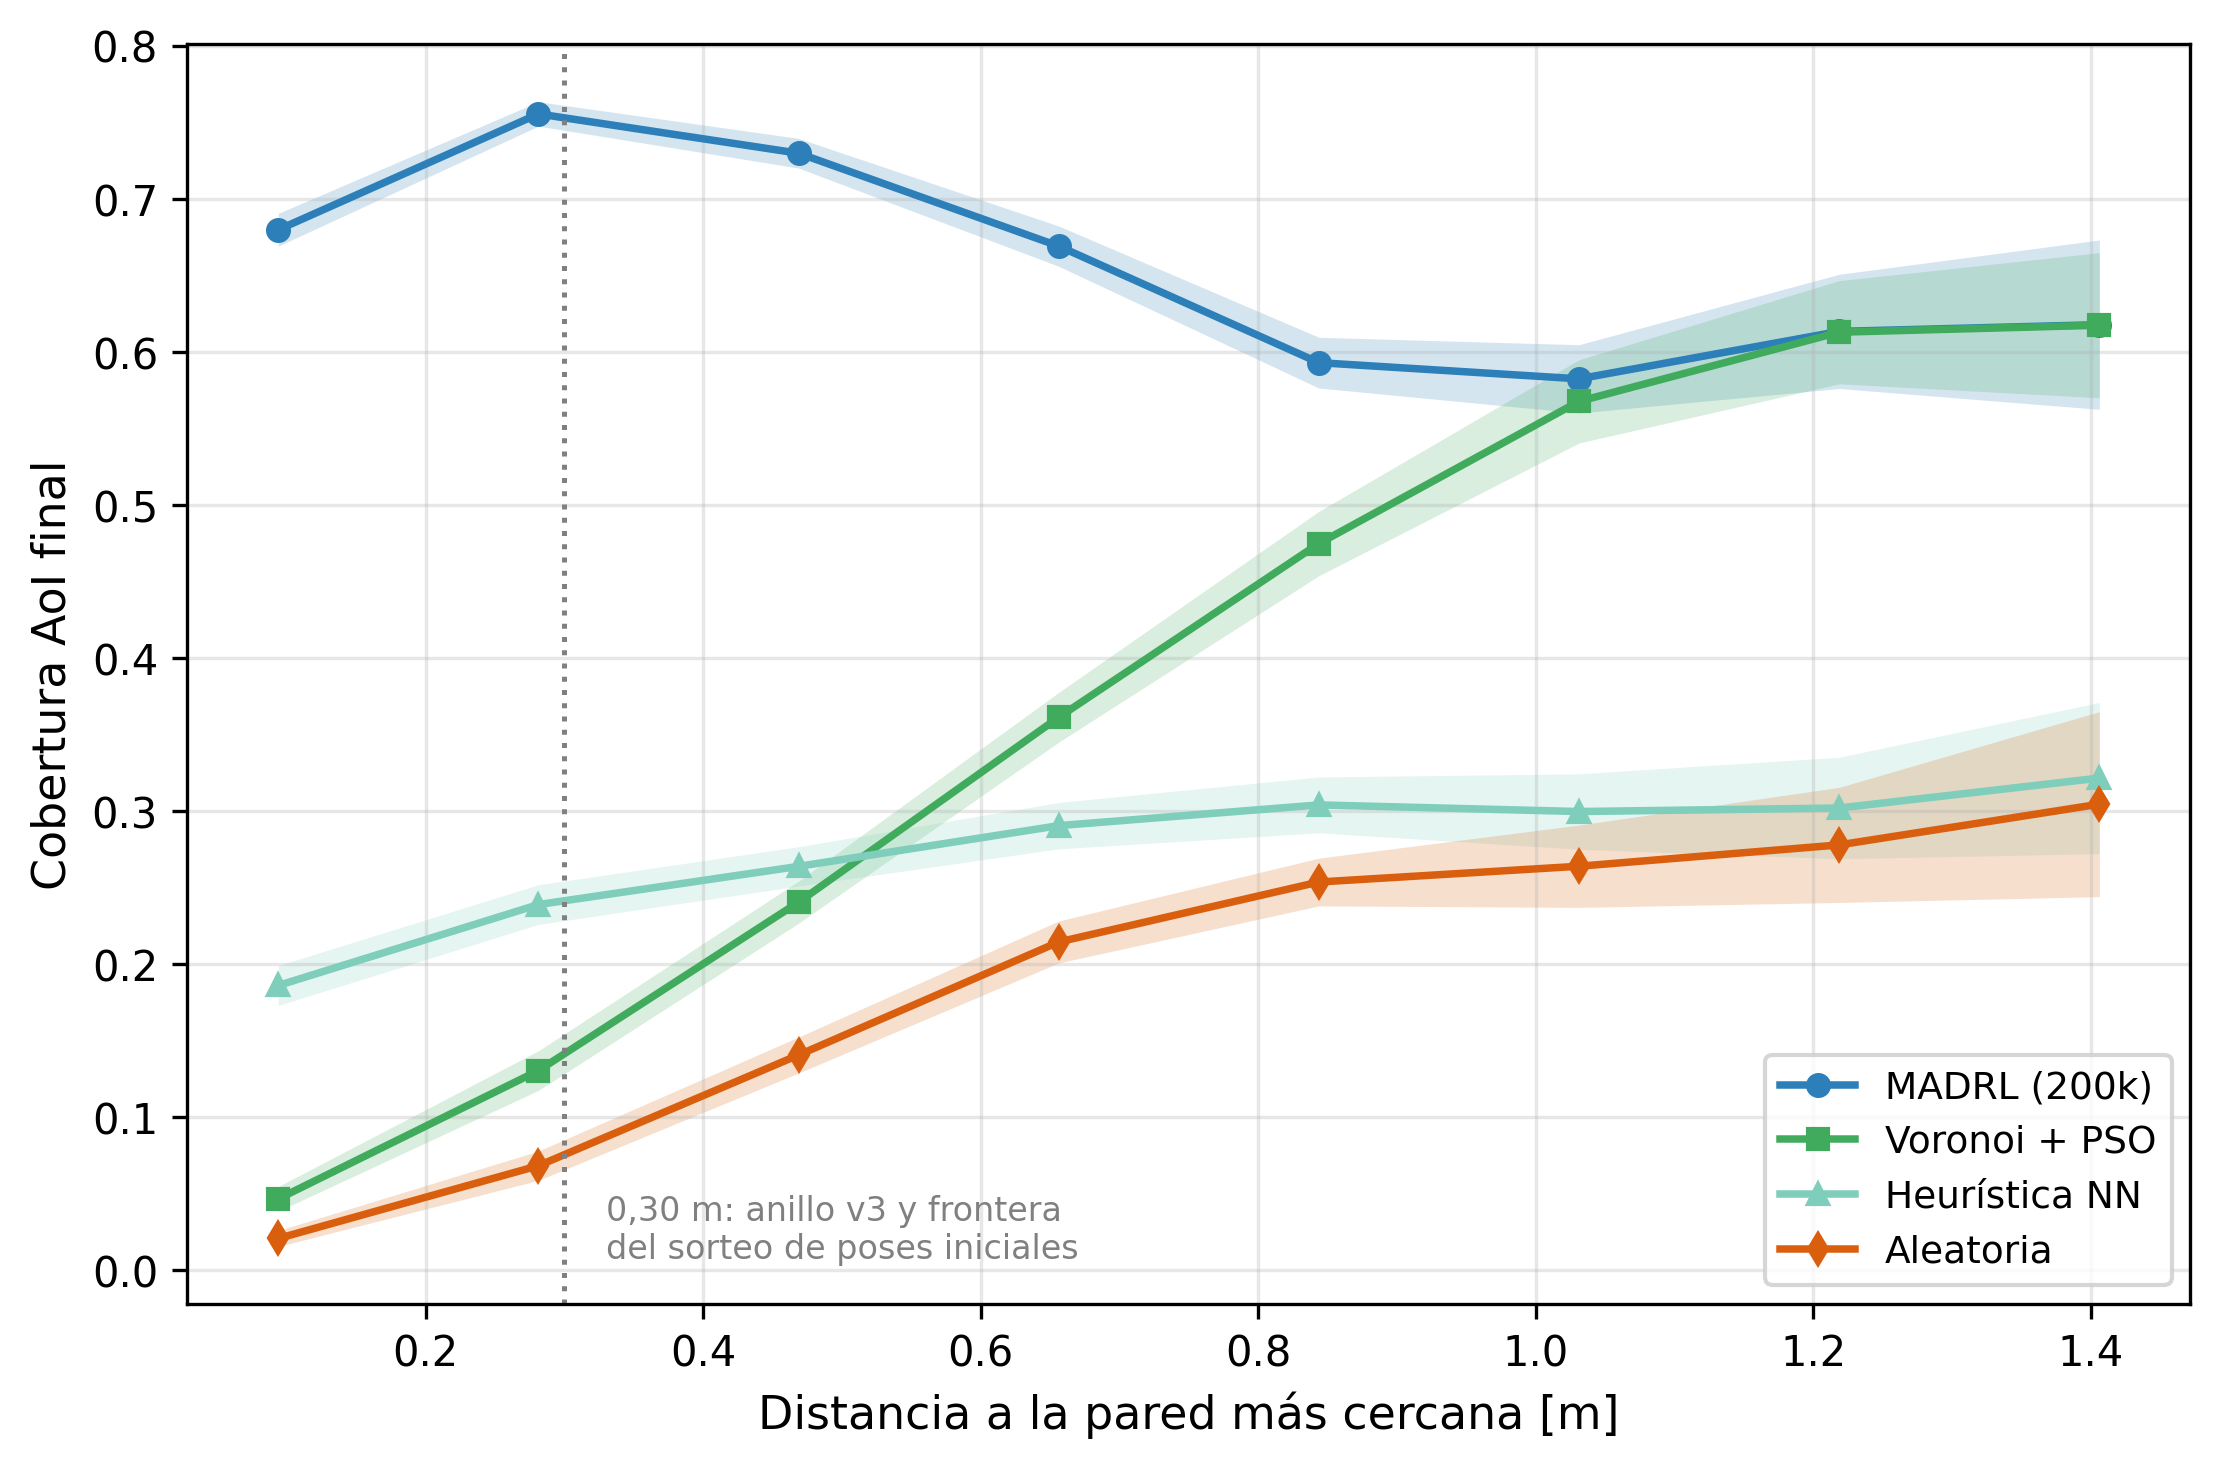
\includegraphics[width=0.90\textwidth]{fig_perfil_radial.png}
    \note{Bandas de cuatro celdas de la cuadrícula. Las regiones sombreadas
          corresponden al intervalo de confianza del $95$\,\% sobre 100 semillas. Elaboración propia.}
    \label{fig:perfil_radial}
\end{figure}

El cruce de pendientes entre la arquitectura MADRL y la de Voronoi con
optimización por enjambre de partículas constituye la representación continua
de los modos de falla opuestos descritos en dicho capítulo. En las dos bandas
más centrales ambas arquitecturas resultan equivalentes, lo cual establece que
la ventaja agregada se obtiene en el perímetro y no en el centro.

% -----------------------------------------------------------------------------
\section{Análisis de asociación entre hiperparámetros y desempeño}
% -----------------------------------------------------------------------------

El análisis de asociación entre hiperparámetros y desempeño admite varias
formulaciones que no resultan equivalentes, y cuya distinción es necesaria para
interpretar los resultados. La cobertura y la tasa de colisiones pueden
evaluarse en el punto de control retenido por cada semilla —que difiere entre
ellas— o en un paso fijo común. El Cuadro~\ref{tab:correlaciones_J} recoge
ambas formulaciones.

\begin{table}[h]
    \centering\captionsetup{width=0.95\linewidth}
    \caption{Correlaciones de rango entre hiperparámetros y desempeño, según
             la magnitud evaluada y el punto de evaluación}
    \begin{tabular}{lcccc}
        \textbf{Hiperparámetro} & \multicolumn{2}{c}{\textbf{En el punto
        retenido}} & \multicolumn{2}{c}{\textbf{A paso fijo (200\,000)}} \\
        & \textbf{Cobertura} & \textbf{Colisiones} & \textbf{Cobertura} &
        \textbf{Colisiones} \\
        \hline
        $\lambda_{\text{cbf}}$ & $0{.}695^{*}$ & $0{.}671^{*}$ & $0{.}144$
            & $0{.}132$ \\
        $\lambda_{\text{ent}}$ & $-0{.}427$ & $-0{.}768^{*}$ & $-0{.}098$
            & $-0{.}182$ \\
        Épocas por actualización & $0{.}344$ & $-0{.}282$ & $0{.}374$
            & $-0{.}288$ \\
        Exponente del horizonte & $\mathbf{-0{.}853^{*}}$ & $-0{.}712^{*}$
            & $\mathbf{-0{.}400^{*}}$ & $-0{.}016$ \\
    \end{tabular}
    \note{El asterisco indica $p < 0{.}05$. Las columnas del punto retenido se
          calculan sobre las 10 pruebas completas; las de paso fijo, sobre
          las 29 semillas individuales. Elaboración propia.}
    \label{tab:correlaciones_J}
\end{table}

\begin{figure}[h]
    \centering\captionsetup{width=0.85\linewidth}
    \caption{Cobertura AoI en función de cada hiperparámetro, evaluada en el
             punto de control retenido}
    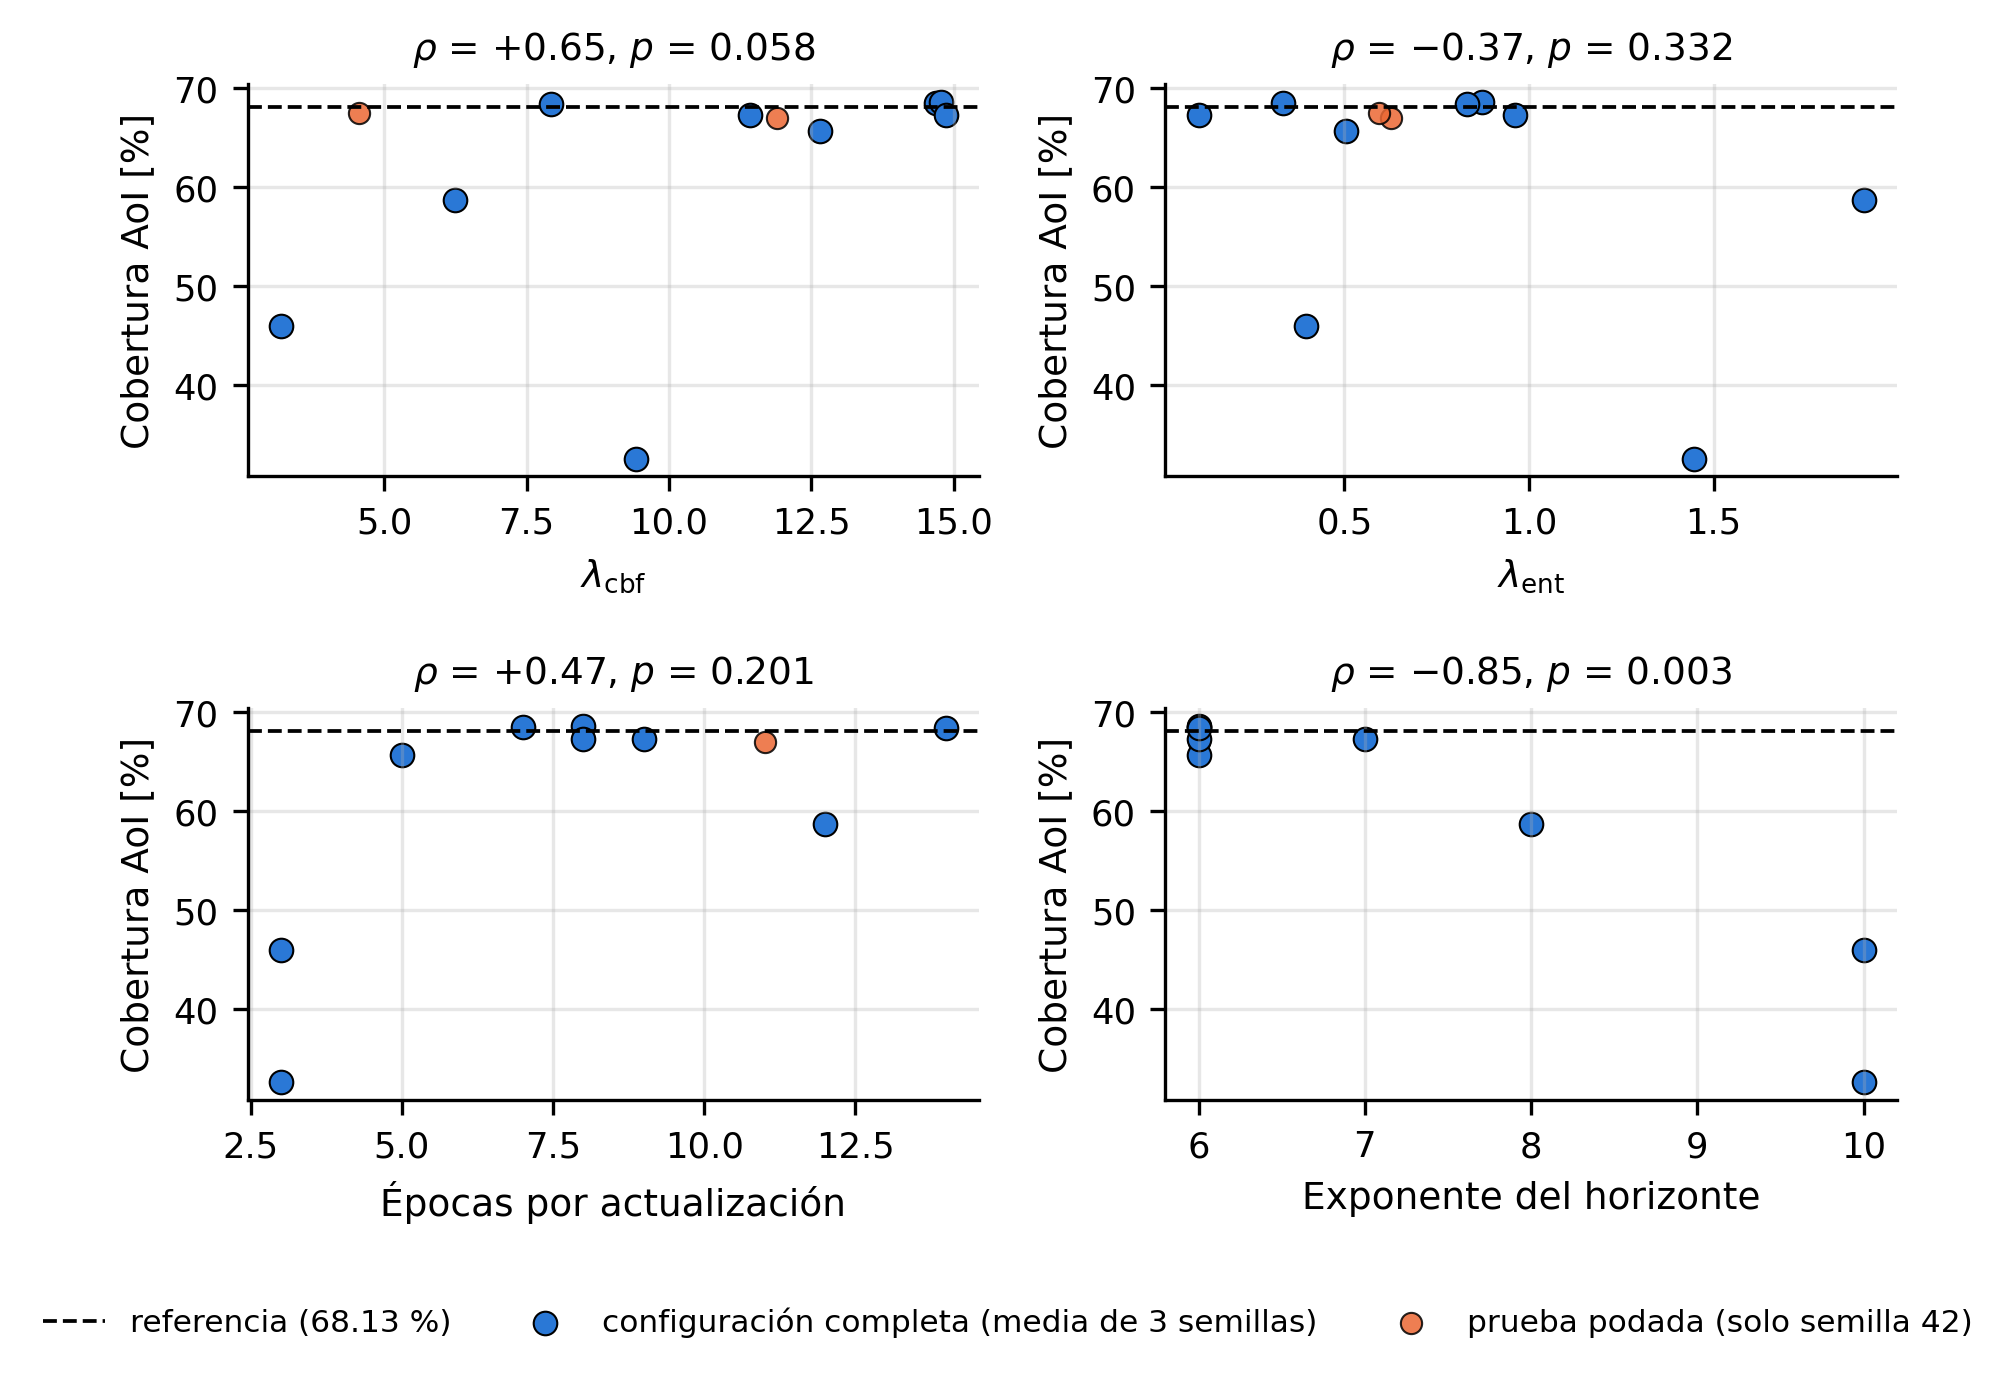
\includegraphics[width=0.95\textwidth]{scatter_hparams_J.png}
    \note{Cada punto azul corresponde a una prueba completa y su ordenada es la
          media de tres semillas. Los coeficientes de los subtítulos se
          calculan únicamente sobre dichas pruebas. Los valores no resultan
          comparables con los del análisis a paso fijo. Elaboración propia.}
    \label{fig:scatter_J}
\end{figure}

La Figura~\ref{fig:scatter_J} muestra la cobertura AoI frente a cada hiperparámetro en el punto de control retenido. El único hiperparámetro cuya asociación tiene el mismo signo en ambas formulaciones es el exponente del horizonte de recolección, con $\rho = -0{.}853$ en el punto retenido y $\rho = -0{.}400$ a paso fijo. Esa asociación es significativa solo en la primera formulación, porque con la corrección de Holm por comparaciones múltiples el coeficiente a paso fijo deja de serlo. El respaldo cualitativo, en cambio, es consistente, ya que las cinco configuraciones
de mejor desempeño emplean horizontes de 64 o 128 pasos, mientras las dos
peores emplean 1024. El número de épocas por actualización no alcanza
significancia en ninguna de las dos formulaciones.

El peso de penalización por proximidad necesita un tratamiento aparte, porque sus dos estimaciones son muy distintas, $\rho = 0{.}695$ en el punto retenido frente a $\rho = 0{.}144$ a paso fijo, para la misma variable dependiente. La diferencia no viene de la magnitud evaluada, sino del punto de evaluación, y tiene dos explicaciones que este diseño no permite separar. La primera es la contaminación por la posición del punto retenido, ya que cada semilla retiene en un paso distinto y la correlación a nivel de prueba mezcla el efecto del hiperparámetro con el del instante en que se observó. La segunda es la covariación con el exponente del horizonte, que en el mismo conjunto de 10 pruebas tiene $\rho = -0{.}853$. El modelo subrogado exploró ambos parámetros juntos y en una zona concentrada, por lo que sus contribuciones no se pueden identificar con 10 observaciones. Por lo tanto, este estudio no tiene potencia para atribuir un efecto al peso de penalización en ninguna dirección.

Las dos formulaciones tienen limitaciones metodológicas. Las correlaciones en el punto retenido están afectadas por la contaminación descrita, cuya magnitud se ve en que una misma configuración registró $0{.}800$, $3{.}633$ y $4{.}933$ colisiones según la semilla, porque cada una retuvo en un paso distinto. Las correlaciones a paso fijo, por su parte, caen en pseudorreplicación, porque las 29 semillas vienen de unas 12 configuraciones. El tamaño de muestra efectivo para un efecto de hiperparámetro es el número de configuraciones y no el de semillas, y los valores de significancia son, por lo tanto, optimistas.


\begin{thebibliography}{1}
\bibitem{huttenrauch2019deep}
M.~Hüttenrauch, A.~Šošić y G.~Neumann, ``Deep reinforcement learning for swarm
systems'', \textit{Journal of Machine Learning Research}, vol.~20, n.º~54,
pp.~1--31, 2019. Disponible en: \url{https://jmlr.org/papers/v20/18-476.html}
\end{thebibliography}

\end{document}
